\chapter[Current Progress]{Current Progress}

\section{Background}

Work started on the \gls{cita} on \gls{chip} project in early 2015. Since then, the research team has developed interactive homework questions as well as tools that can track and analyze student progress. This parallel development of problems and analysis tools will ensure that the research team can continuously improve the system over many semesters in a structured way. It also ensures that the research team can react to changing requirements in an efficient manner.

\section{Development of CITA}

In order to create a consistent and effective tutorial system, I have divided the structure of \gls{cita} up into three main parts - Shallow \gls{cita}, Immersive \gls{cita}, and Postscripts. A single homework problem usually has all three of these pieces, but might omit one if it is not appropriate for the analysis. None of these individual pieces are a solution on their own; it is only when they are combined in the proper way does the interactive analysis become useful.

\subsection{Shallow CITA}

Shallow \gls{cita} anticipates and corrects simple mistakes in student answers. This might include unit errors, misreading the question, or sign errors. It is intended to help students correct simple mistakes that would otherwise lose them easy points. In other words, Shallow \gls{cita} is meant to catch all of the ``low hanging fruit'' - the easy problems that can be solved with minimal trouble.

Shallow \gls{cita} is very important in our system because it filters out mistakes that come from superficial errors and mistakes that come from a true misunderstanding of the material. We do not want to force students to go through a full tutorial if they have only made a simple sign error. This would lead to dissatisfaction with the system and perhaps even a reluctance to use it in the future.

Shallow \gls{cita} does not transition the user to a new interface. Therefore, there is not enough space on the screen to truly set up a new model or derive new equations. Instead, it simply displays a short message (one paragraph or less) so that the user can make minor corrections to his or her analysis and continue with the remainder of the homework assignment.

\subsection{Immersive CITA}

Immersive \gls{cita} gives a step-by-step walkthrough of the specific homework problem, providing students with the structure that they need to complete tough homework questions. Unlike other scaffolding systems, it does not simply give an algorithmic list of steps. Instead, students have to answer questions and work through the example in order to get the answer. Ideally, Immersive \gls{cita} will provide multiple paths for students to take through each example.

Immersive \gls{cita} is not supposed to be an artificial intelligence. Instead, it provides the structure that students need to think about a problem. It encourages discussion over algorithms. Thus, immersive \gls{cita} guides students through problems so that they have the background knowledge needed to participate in discussions. If students cannot solve the problem even after going through the full tutorial, Immersive \gls{cita} will refer them to a professor or teaching assistant with specific questions to ask.

\subsubsection{Branching Structures}

The crux of our study is to determine how different branching structures affect student learning. In Table \ref{tab:structures} I give a summary of the structures that have been developed and implemented in the system as of now.

Table \ref{tab:questionStats} shows our current progress and future goals for developing branching questions. In Figure \ref{fig:questionStatistics} I have plotted the number of questions that use the different types of branching systems in the homework. Notice how the research team has increased the number of linear and branching questions from spring to summer. Linear questions include those with only one single hint or a linear path. Branching questions are those that involve tree, recombination, and dead end structures.

\pagebreak

\begin{footnotesize}
\begin{table}
  \centering
  \begin{tabular}{|p{2.5cm}|p{5.4cm}|p{4.4cm}|}
    \hline
    \textbf{Structure} & \textbf{Description} & \textbf{Examples}\\
	\hline
	No Structure & Some problems do not require the sophistication of a branching structure due to their simple nature. Other problems are meant to assess student performance, so a branching structure would skew results.
 & Weekly Reading Quiz Problems, Diagnostic Problems, Practice Test Problems\\
	\hline
	Single Hint & This structure is useful for problems that are relatively easy to do after students realize one key concept. Once students realize the ``trick'' the remaining analysis is straightforward. & Drawing a Good Diagram Before Using Superposition, Rayleigh Criteria, Geometric Optics\\
	\hline
	Linear & These are problems that have one preferred solution that is taught in an introductory physics student. We try to avoid using this structure as much as possible. However, when it is used, checkbox and numerical questions point out common misconceptions. & Thin Film Interference, Wave Equation\\
	\hline
	Recombination & Students realize that two seemingly different paths of logic are related. This structure is great for derivations because it shows students that there is more than one way to get from point A to point B.
 & Coulomb’s Law vs. Gauss’s Law for Continuous Charge Distributions\\
	\hline
	Tree & Each step in the analysis leads to new, unique steps. These might branch out into further unique steps. Depending on the analysis, students may get seemingly different answers. & Electric Circuits, Using Different Coordinate Systems in Some Problem\\
	\hline
	Dead End & Students analyze a problem in a reasonable way, learning later why their thought process was flathe research teamd. This structure lets students make mistakes - one of the most important parts of learning. & Integrating With Respect to Certain Variables Rather Than Others, Right Hand Rules\\
	\hline
  \end{tabular}
  \caption{Branching Structures}
  \label{tab:structures}
\end{table}
\end{footnotesize}

\begin{figure}
	\centering
	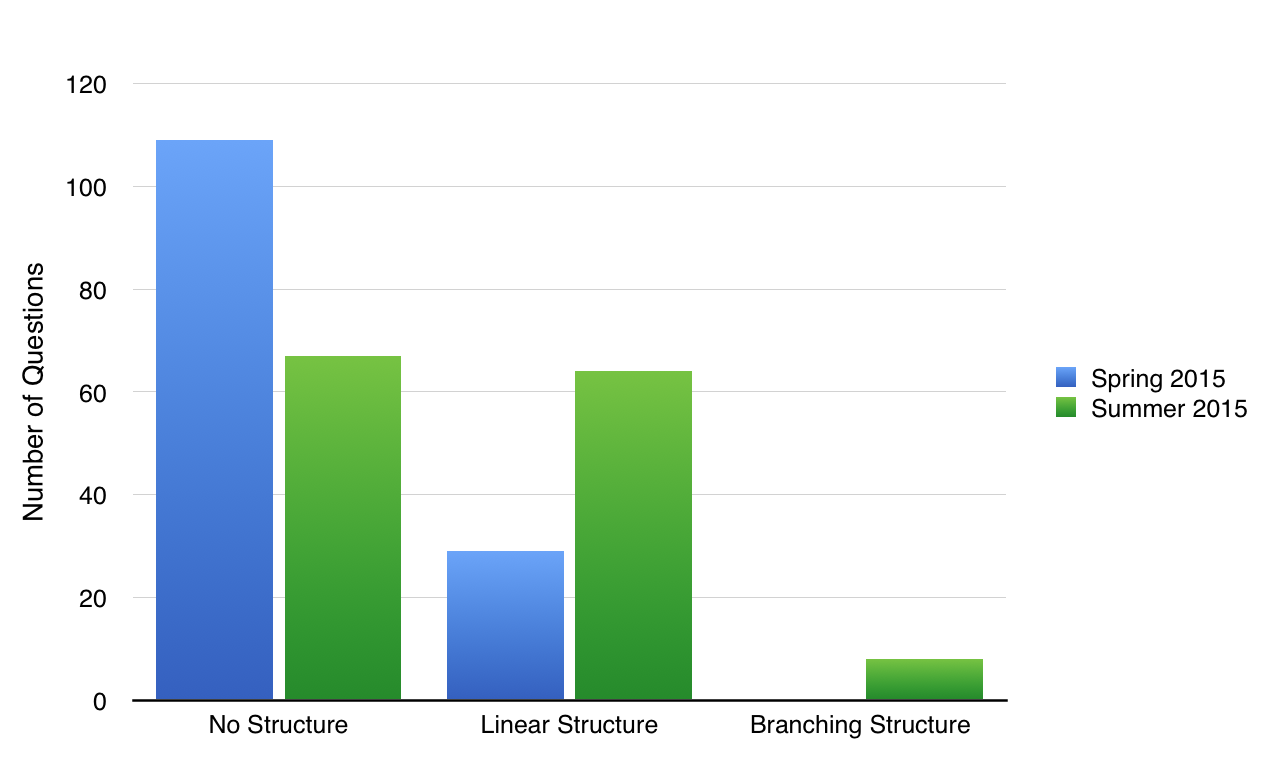
\includegraphics[width=6in]{img/chapter4/question_statistics}
	\caption[The Number of Linear and Branching Questions Implemented in the PHYS 24100 Homework]{The Number of Linear and Branching Questions Implemented in the PHYS 24100 Homework}
  \label{fig:questionStatistics}
\end{figure}

\begin{table}
  \centering
  \begin{tabular}{|l|l|l|l|}
    \hline
    \textbf{Structure} & \textbf{Spring 2015} & \textbf{Summer 2015} & \textbf{Fall 2015 Goals}\\
	\hline
	No Structure & 109 & 67 & 20\\
	\hline
	Linear & 29 & 64 & 80\\
	\hline
	Branching & 0 & 8 & 40\\
	\hline
  \end{tabular}
  \caption{Question Statistics and Goals}
  \label{tab:questionStats}
\end{table}

\subsection{Postscripts}

After a student completes a homework problem, he or she is presented with one or two qualitative questions that expand on the topics covered in the homework. For example, after solving a circuit question, the followup question might ask students how the problem would change if the battery was connected in reverse. These postscript questions are not counted for a grade; instead, they are meant to encourage deeper thought about the problem. This deeper thought about the homework question is meant to expand student’s knowledge of the concepts at hand.

This section can be used to ask slightly more obscure questions that would not usually be fitting for a graded homework. For example, we might ask the introductory physics students to speculate how Maxwell's equations would change if magnetic monopoles did exist. Or we might ask the students to estimate the electric potential energy needed to launch a projectile to the moon. Once again, these questions are not meant to be harshly graded - only to make the students think about the concepts in the homework.

\section{Development of Analysis Tools}

\subsection{CHIP}

\gls{chip} has a useful set of built in statistical analysis tools. Most of the quantiative analysis that the research team plan to do will take place through the \gls{chip} \gls{gui}. However, \gls{chip} does not support operations like Student t-Tests or ANOVA. For now, these additional operations will be done using R or an equivalent statistical analysis program. They might be added to \gls{chip} at a later date.

\subsection{Muffin}

Over the course of this project, the research team will have to deal with data from a variety of sources. For example, CSV data from the \gls{chip} website might have to be parsed with JSON data from the Piazza website. Audio data from focus group transcripts might have to be compared to written data from notes taken by teaching assistants. We need a simple and efficient way to translate one data format into another.

I have written an open-source data analysis toolbox called Muffin that will handle this information. Muffin is a set of Ruby functions that will read and write data to a format appropriate for our study. The source code for Muffin is hosted on \index{Ruby Gems}Ruby Gems as well as on my personal \index{GitHub}GitHub page.

Muffin is simply a toolbox that converts data from one format to another. It does not store anything or conduct analysis in any way. Thus, privacy is maintained, even when the Muffin source code is freely distributed online.

\section{Current Results}

\subsection{BEMA Results}

We used the \gls{bema} exam to conduct a preliminary analysis of the effectiveness of the \gls{cita} on \gls{chip} system. In \ref{fig:bemaSp15} I plot the pre- and post-test scores of students taking the exam in the spring 2015 semester. These students are in the on-campus, PHYS 24100 course. In Figure \ref{fig:bemaSu15} I plot the pre- and post-test scores of students taking the exam in the summer 2015 semester. Tables \ref{tab:statsSp15} and \ref{tab:statsSu15} provide a statistical analysis of the data. We see that the samples in each semester are not normally distributed. Using a Wilcoxon Signed-Rank test, we find that difference in the means between the pre- and post-test are statistically significant in both the spring and summer classes. The effect size of these differences is d = 0.588.

\begin{figure}
	\centering
	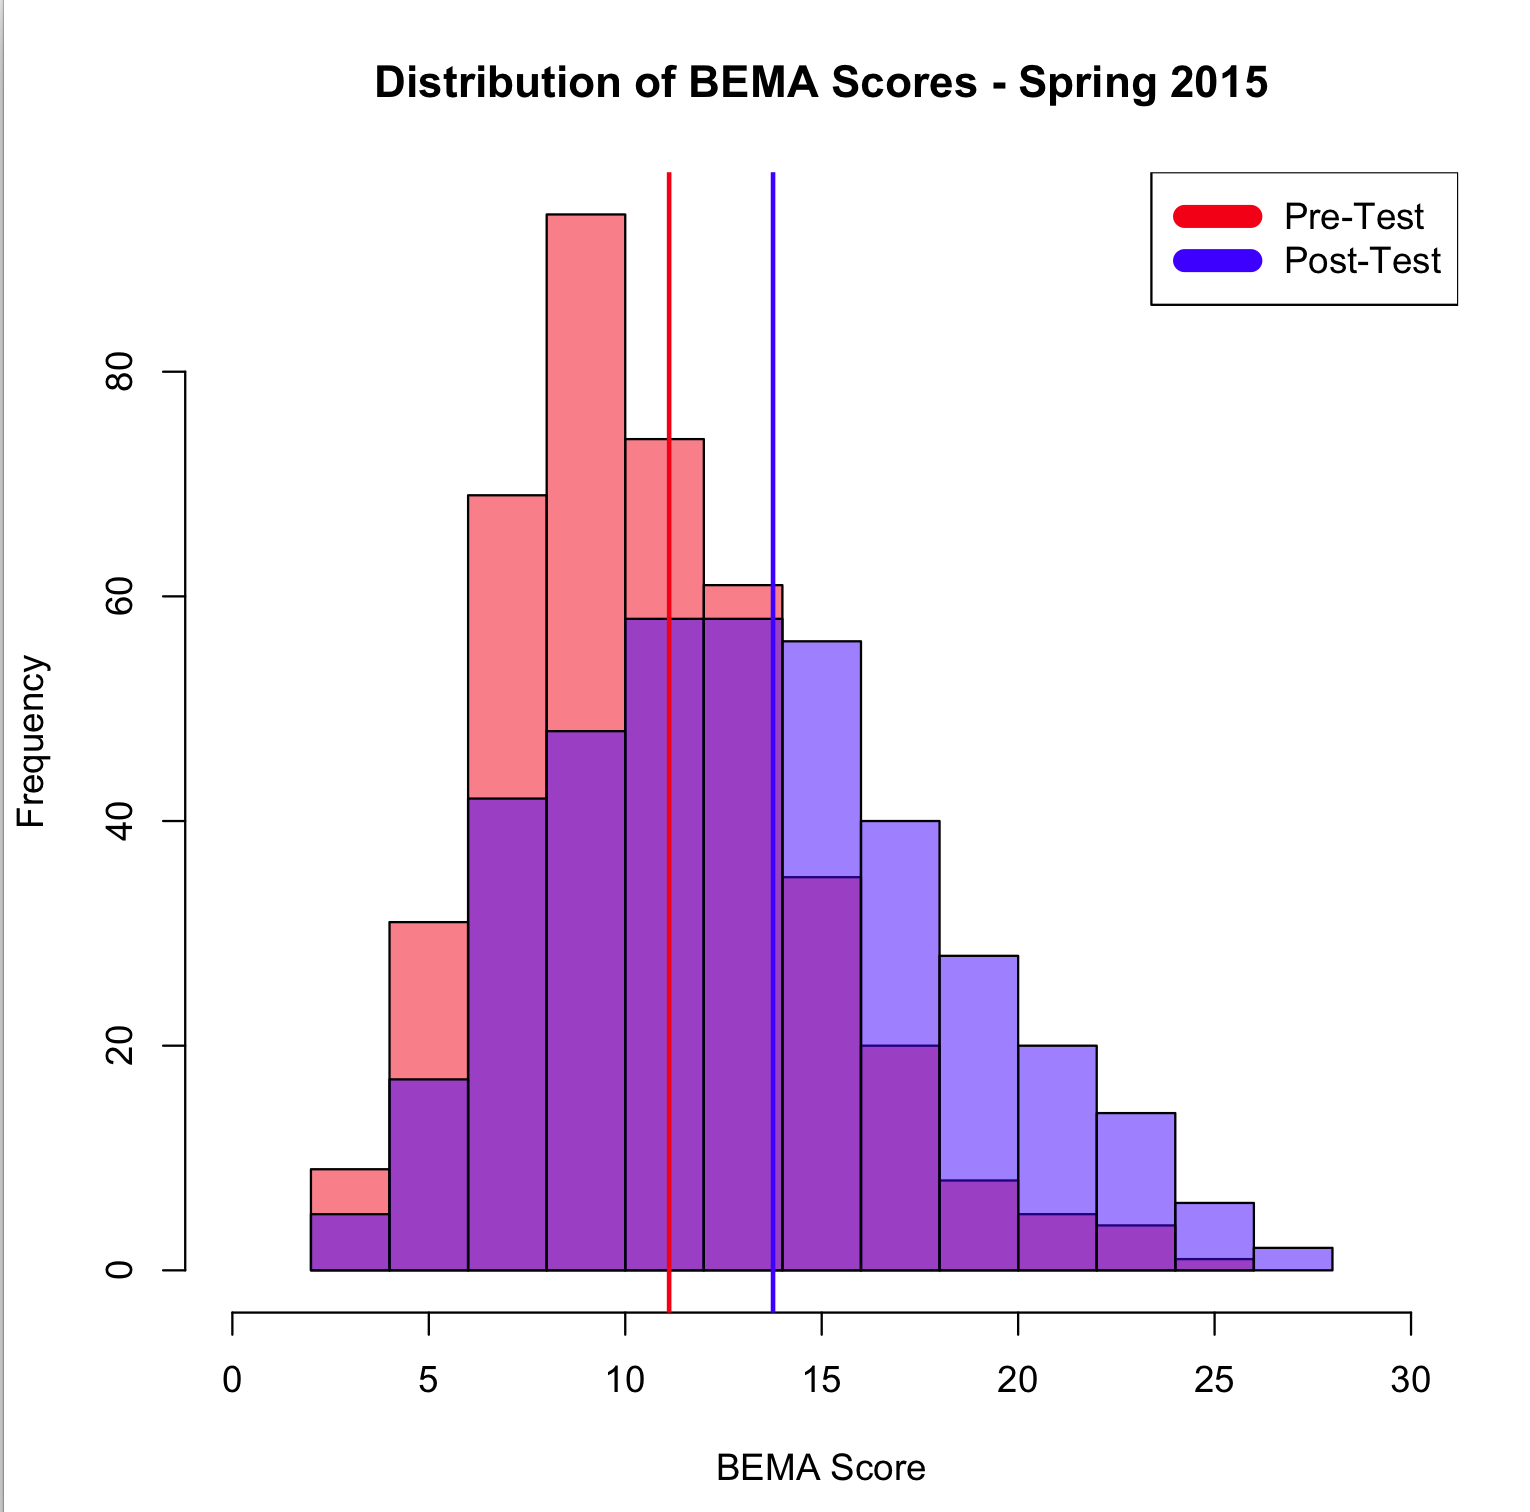
\includegraphics[width=6in]{img/chapter4/bema_spring_2015}
	\caption[BEMA Scores for the Spring 2015 PHYS 24100 Class]{BEMA Scores for the Spring 2015 PHYS 24100 Class}
  \label{fig:bemaSp15}
\end{figure}

\begin{small}
\begin{table}
  \centering
  \begin{tabular}{|l|l|}
    \hline
    \textbf{Statistic} & \textbf{Value}\\
	\hline
	Mean of Pre-Test & 11.117 \\
	\hline
	Mean of Post-Test & 13.761 \\
	\hline
	Standard Deviation of Pre-Test & 3.923 \\
	\hline
	Standard Deviation of Post-Test & 5.030 \\
	\hline
	Shapiro-Wilk Normality Test of Pre-Test & p-value = 9.24e-08 \\
	\hline
	Shapiro-Wilk Normality Test of Post-Test & p-value = 0.000138 \\
	\hline
	Wilcoxon Signed-Rank Test of Pre-Test and Post-Test & p-value = 9.74e-15 \\
	\hline
	Cohen's D of Pre-Test and Post-Test & 0.588 \\
	\hline
  \end{tabular}
  \caption{Spring 2015 BEMA Statistics}
  \label{tab:statsSp15}
\end{table}
\end{small}

\begin{figure}
	\centering
	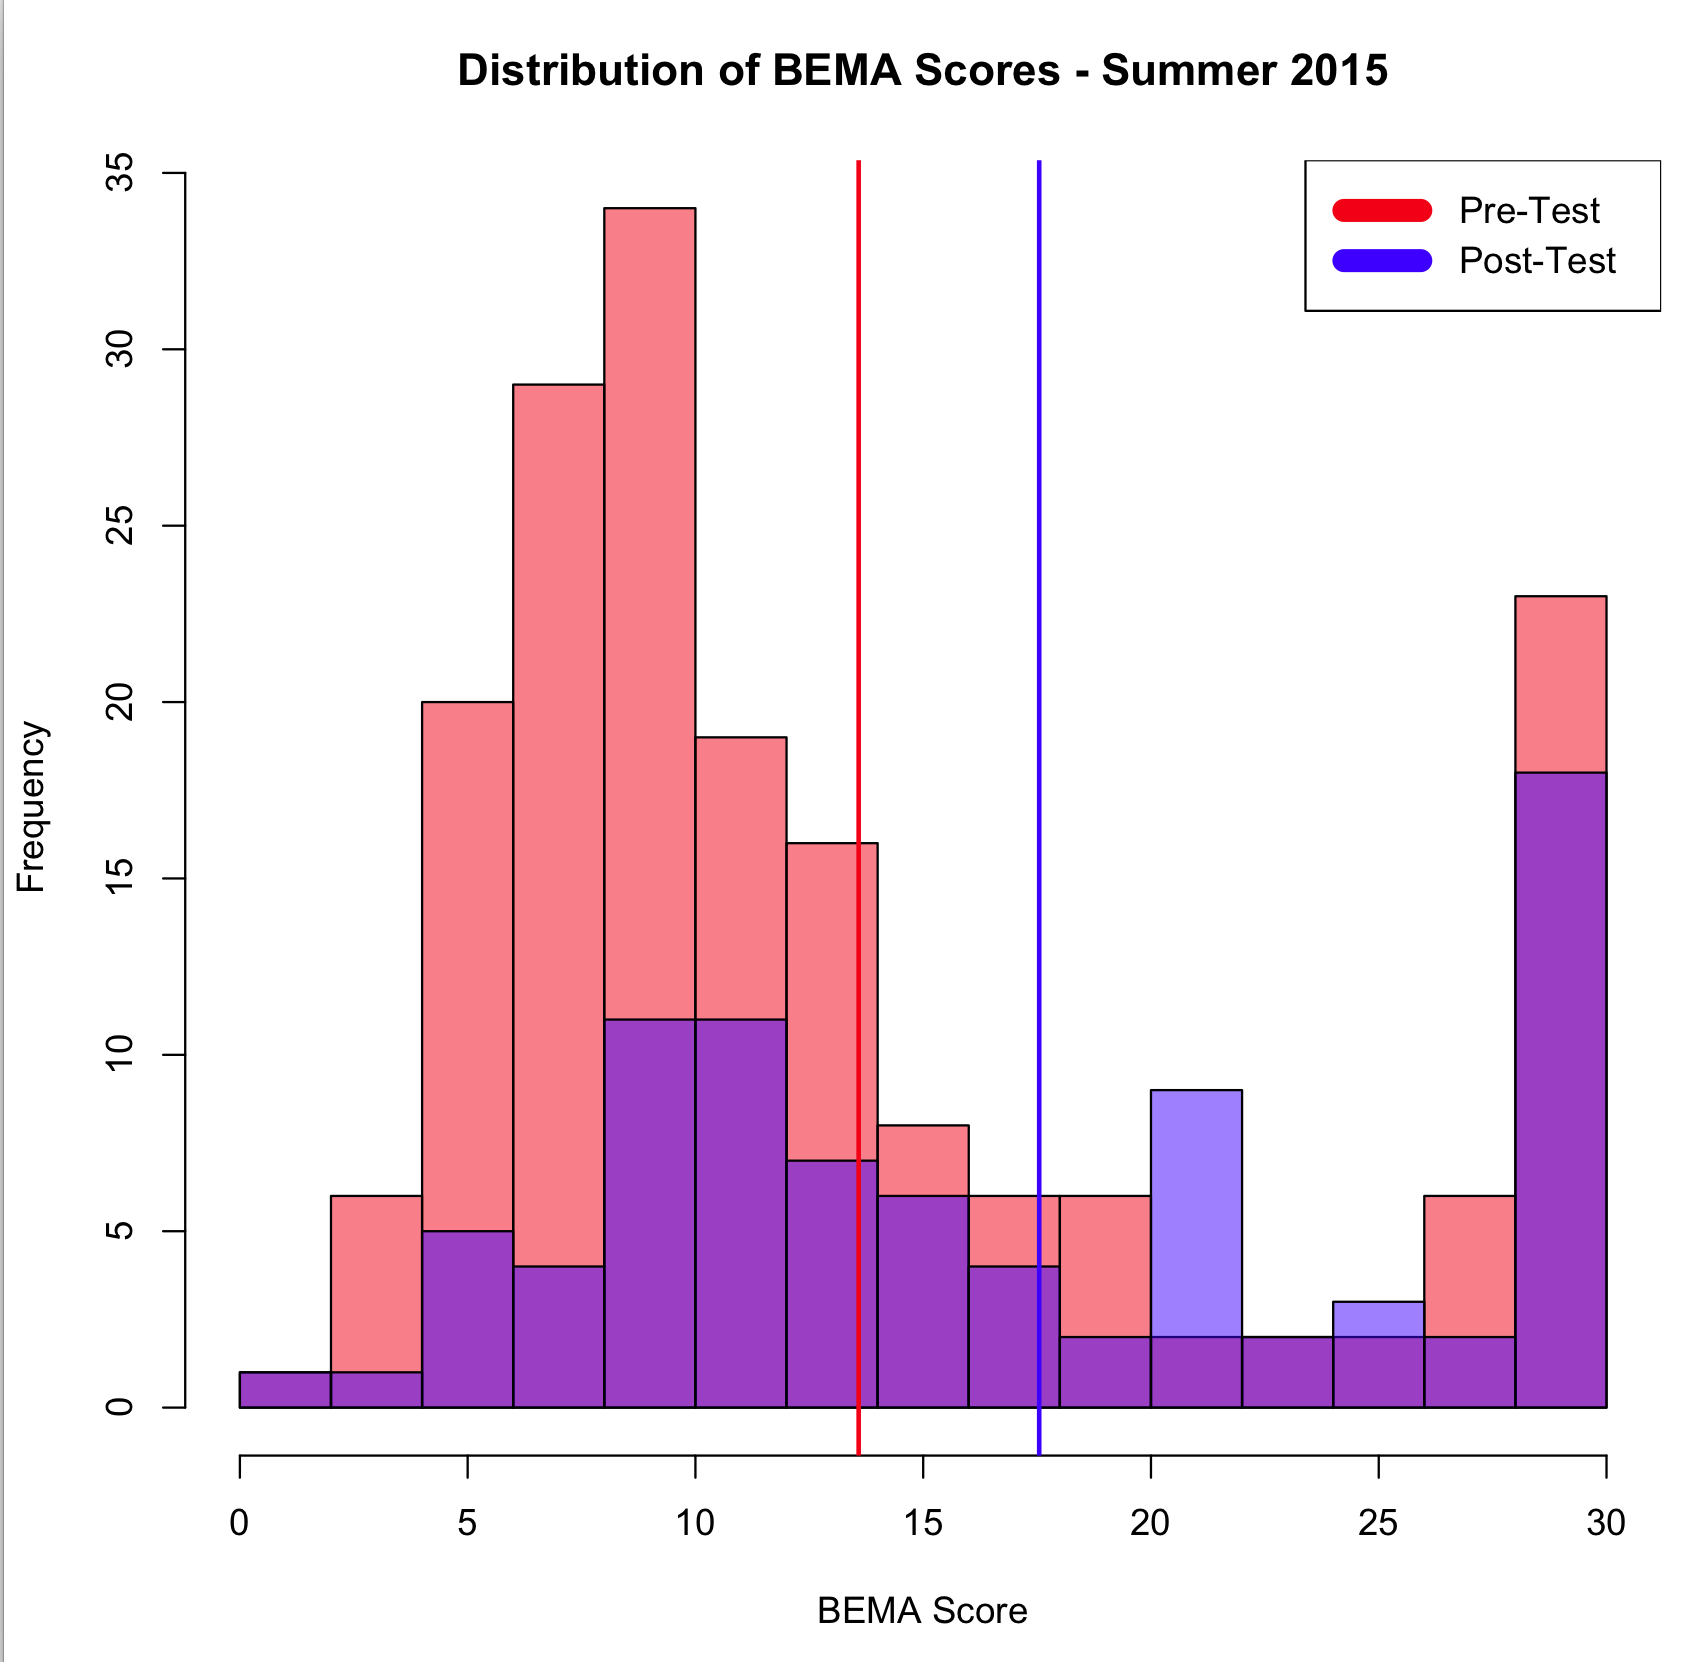
\includegraphics[width=6in]{img/chapter4/bema_summer_2015}
	\caption[BEMA Scores for the Summer 2015 PHYS 24100 Class]{BEMA Scores for the Summer 2015 PHYS 24100 Class}
  \label{fig:bemaSu15}
\end{figure}

\begin{small}
\begin{table}
  \centering
  \begin{tabular}{|l|l|}
    \hline
    \textbf{Statistic} & \textbf{Value} \\
	\hline
	Mean of Pre-Test & 13.583 \\
	\hline
	Mean of Post-Test & 17.547 \\
	\hline
	Standard Deviation of Pre-Test & 8.169 \\
	\hline
	Standard Deviation of Post-Test & 8.500 \\
	\hline
	Shapiro-Wilk Normality Test of Pre-Test & p-value = 1.599e-12 \\
	\hline
	Shapiro-Wilk Normality Test of Post-Test & p-value = 1.332e-05 \\
	\hline
	Wilcoxon Signed-Rank Test of Pre-Test and Post-Test & p-value = 4.916e-05 \\
	\hline
	Cohen's D of Pre-Test and Post-Test & 0.479 \\
	\hline
  \end{tabular}
  \caption{Summer 2015 BEMA Raw Statistics}
  \label{tab:statsSu15}
\end{table}
\end{small}

It is difficult to make a comparison of the spring and summer classes based on the raw scores alone. The best way to compare the scores between the two classes is to compare the average gains of students rather than the \gls{bema} averages themselves. The Hake or gain factor is calculated using the following formula:

\begin{equation}
	g = \frac{Post - Pre}{31 - Pre}
\end{equation}

Note that the 31 in the denominator comes from the fact that the maximum score on the \gls{bema} exam is 31 points. In Figure \ref{fig:hakeFull} I plot the Hake factors for the two semesters. In the plots, I eliminate one outlier from the summer 2015 course that had a Hake factor of -22.

\begin{figure}
	\centering
	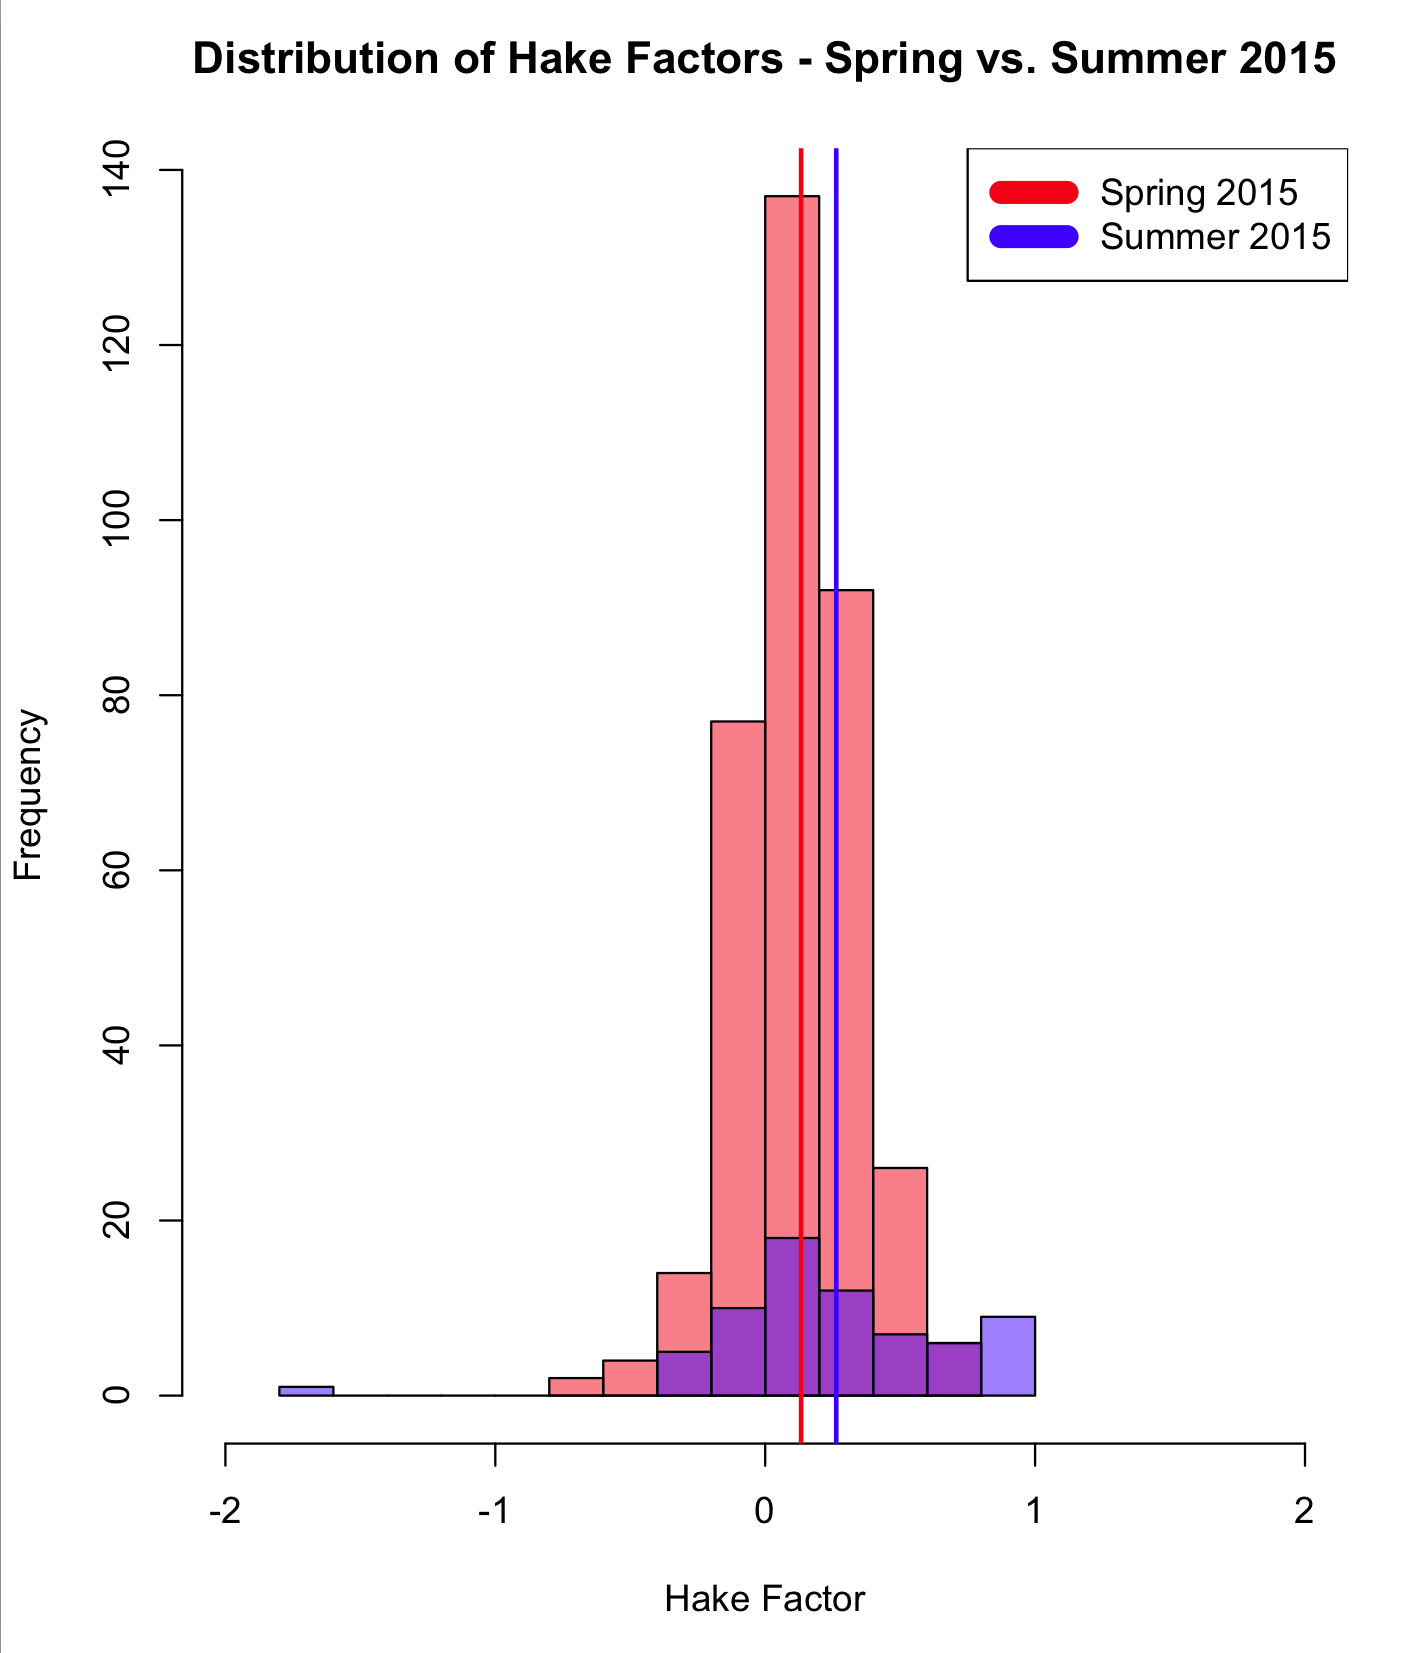
\includegraphics[width=6in]{img/chapter4/hake_spring_vs_summer_full}
	\caption[Comparison of Hake Factors on the BEMA Between Spring and Summer 2015]{Comparison of Hake Factors on the BEMA Between Spring and Summer 2015}
  \label{fig:hakeFull}
\end{figure}

During the summer, the research team noticed a lot of scores that seemed very inflated. We suspect that many students were cheating on the \gls{bema} exam since they could take it online without any supervision. This was not a problem for the spring 2015 PHYS 24100 class because they all took the exam under closely monitored conditions. Thus, in order to better compare the Hake factors, I eliminte all data points from the summer where a student's pre-test score was 27 or higher. The new plot is shown in Figure \ref{fig:hakeFiltered} and the statistical analysis is shown in Table \ref{tab:compareSpSu15}.

\begin{figure}
	\centering
	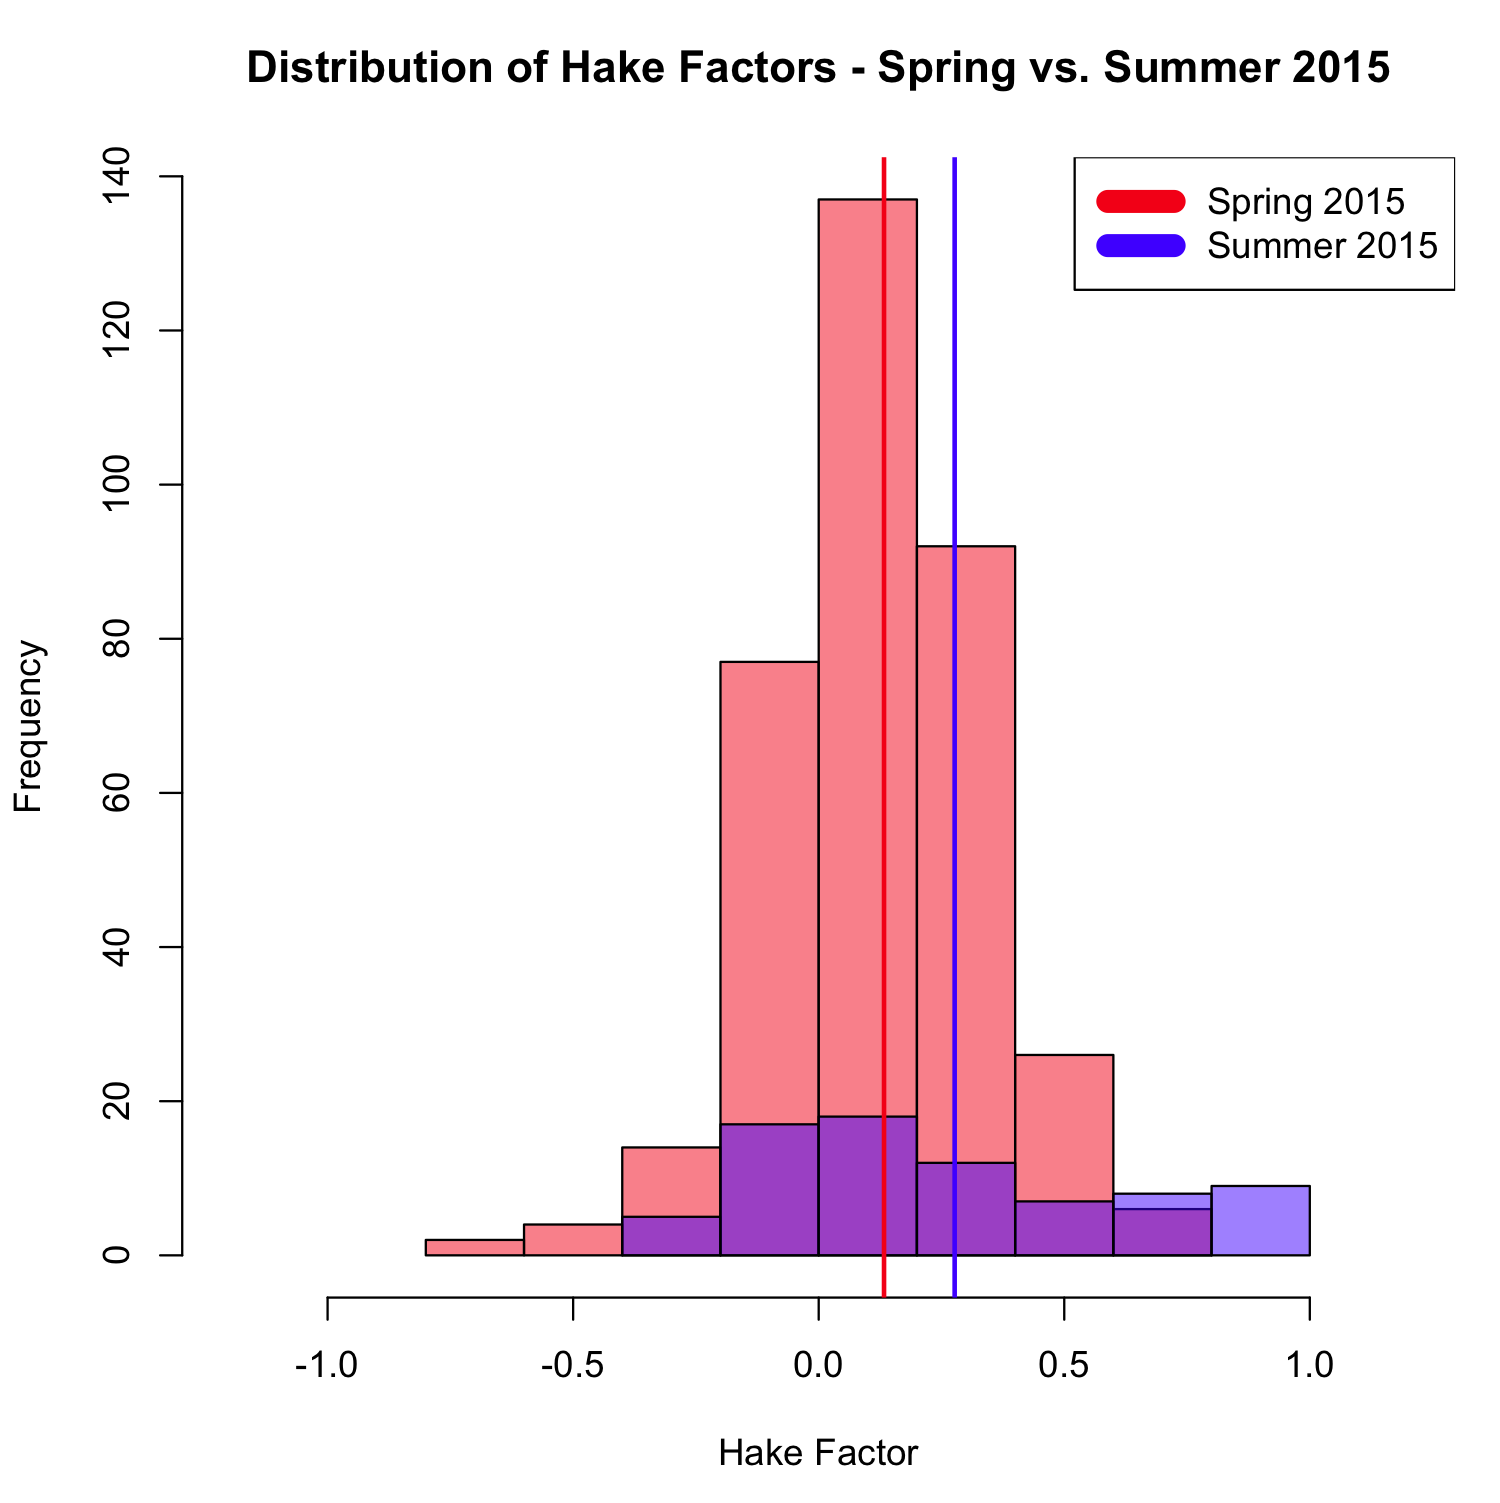
\includegraphics[width=6in]{img/chapter4/hake_spring_vs_summer_filtered}
	\caption[Comparison of Hake Factors on the BEMA Between Spring and Summer 2015, Filtered to Eliminate Outliers and Pre-Test Grades Over 26/31 Points ]{Comparison of Hake Factors on the BEMA Between Spring and Summer 2015, Filtered to Eliminate Outliers and Pre-Test Grades Over 26/31 Points}
  \label{fig:hakeFiltered}
\end{figure}

\begin{small}
\begin{table}
  \centering
  \begin{tabular}{|l|l|}
    \hline
    \textbf{Statistic} & \textbf{Value} \\
	\hline
	Mean of Spring Hake Factors & 0.133 \\
	\hline
	Mean of Summer Hake Factors & 0.263 \\
	\hline
	Standard Deviation of Spring Hake Factors & 0.208 \\
	\hline
	Standard Deviation of Summer Hake Factors & 0.440 \\
	\hline
	Shapiro-Wilk Normality Test of Spring Hake Factors & p-value = 6.683e-05 \\
	\hline
	Shapiro-Wilk Normality Test of Summer Hake Factors & p-value = 8.509e-06 \\
	\hline
	Wilcoxon Signed-Rank Test of Hake Factors & p-value = 0.009334 \\
	\hline
	Cohen's D of Hake Facrors & 0.503 \\
	\hline
  \end{tabular}
  \caption{Spring vs. Summer 2015 Hake Factors, filtering out any data with a pre-test score above 26/31.}
  \label{tab:compareSpSu15}
\end{table}
\end{small}

On first glance, the summer 2015 semester outperformed the spring 2015 semester. Although the initial results for the \gls{bema} look promising, we need to be careful. The spring and summer sections of PHYS 24100 are two very different classes with two very different student bodies. The spring semester is a more traditional student body while the summer semester has the advantage of the internet as a reference (all of the students were online during the summer 2015 semester). Thus, more testing is needed to see if these results truly hold up.

I also plot the \gls{bema} scores for the spring and summer semesters versus scores on the first and second exams (Figures \ref{fig:bemaVsExOneSp15}, \ref{fig:bemaVsExTwoSp15}, \ref{fig:bemaVsExOneSu15}, and \ref{fig:bemaVsExTwoSu15}). Notice that the first and second exam for the summer classes have generally higher scores than the on-campus sections in the spring. We see this because the online classes can use their books, notes, and the internet to work on their exams.

\begin{figure}
	\centering
	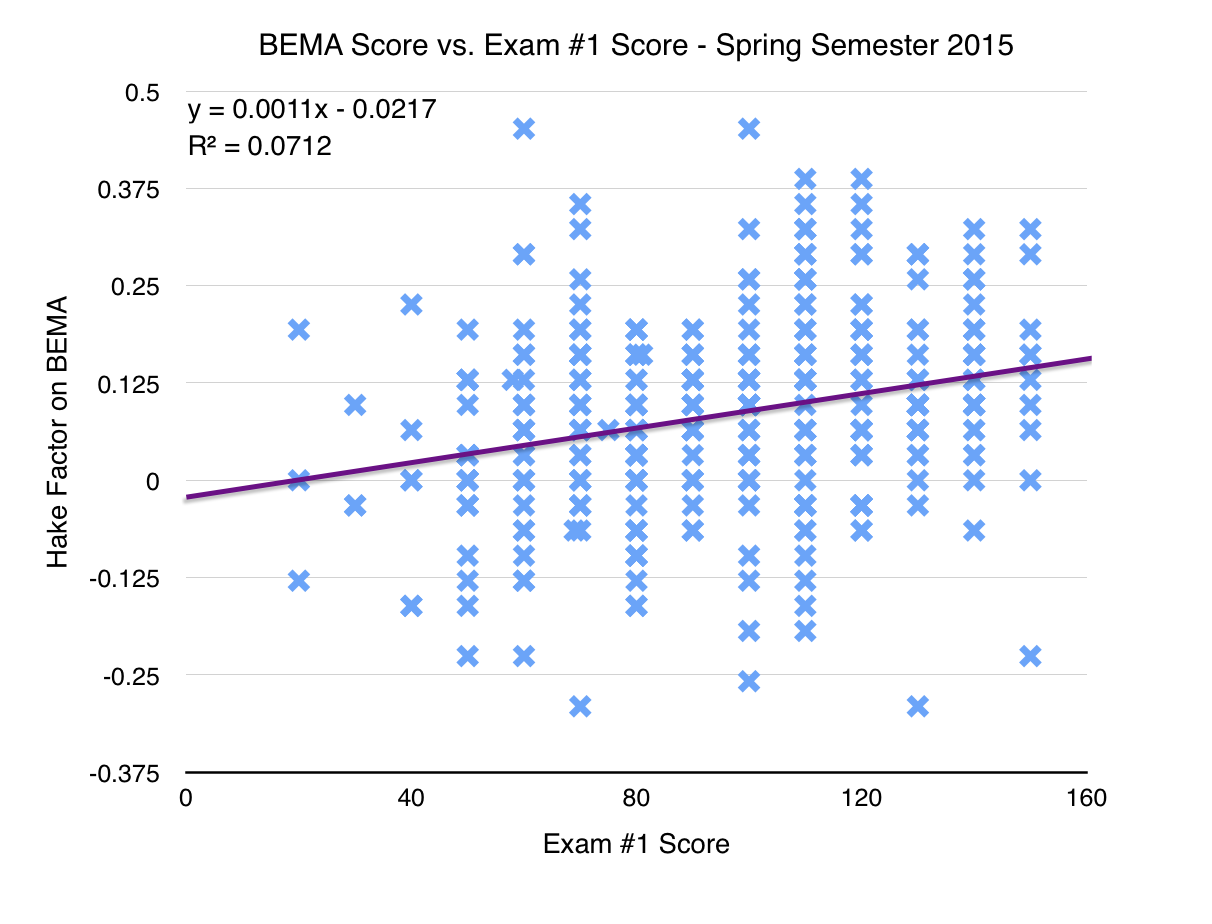
\includegraphics[width=6in]{img/chapter4/bema_vs_ex1_sp15}
	\caption[BEMA Hake Factor vs. Exam \#1 Scores]{BEMA Hake Factor vs. Exam \#1 Scores}
  \label{fig:bemaVsExOneSp15}
\end{figure}

\begin{figure}
	\centering
	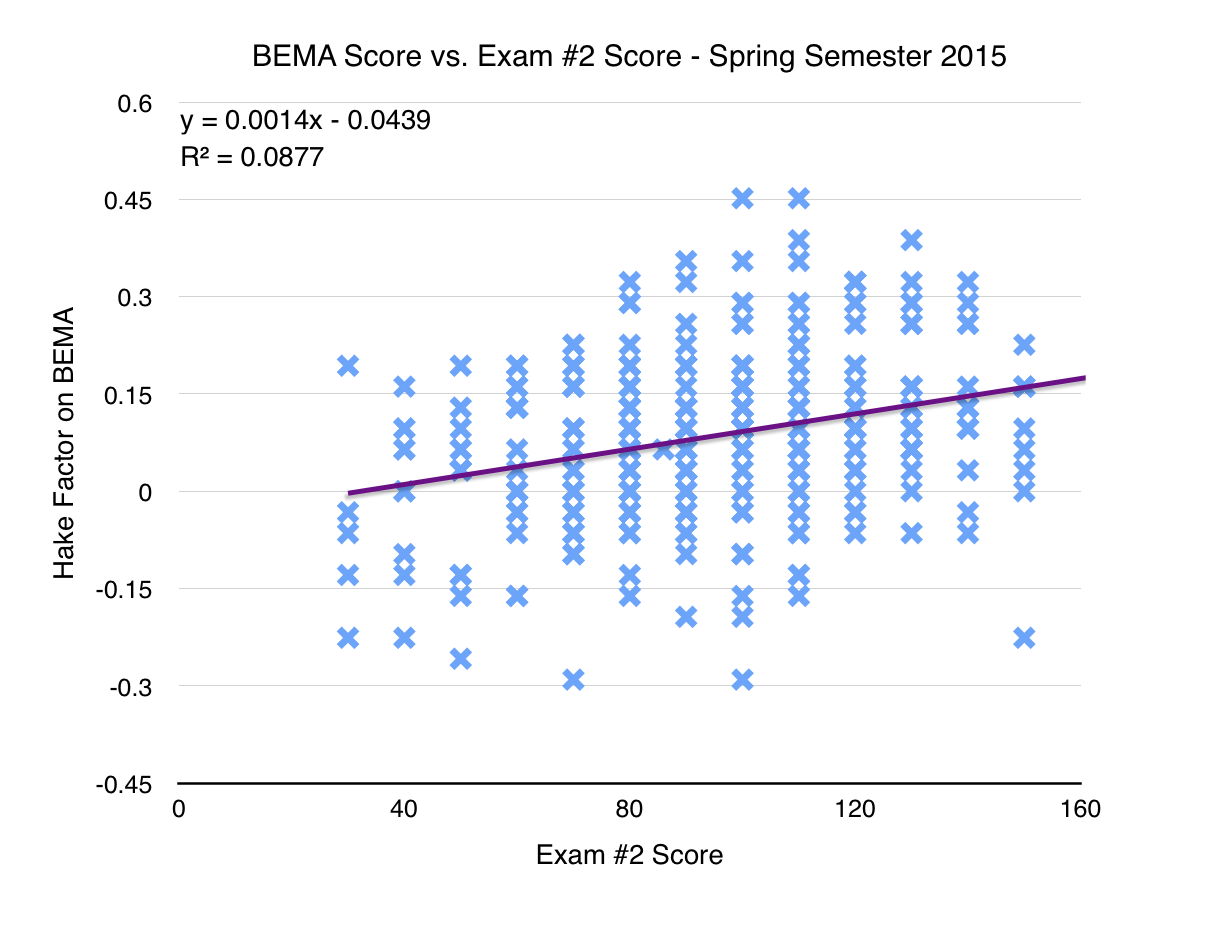
\includegraphics[width=6in]{img/chapter4/bema_vs_ex2_sp15}
	\caption[BEMA Hake Factor vs. Exam \#2 Scores]{BEMA Hake Factor vs. Exam \#2 Scores}
  \label{fig:bemaVsExTwoSp15}
\end{figure}

\begin{figure}
	\centering
	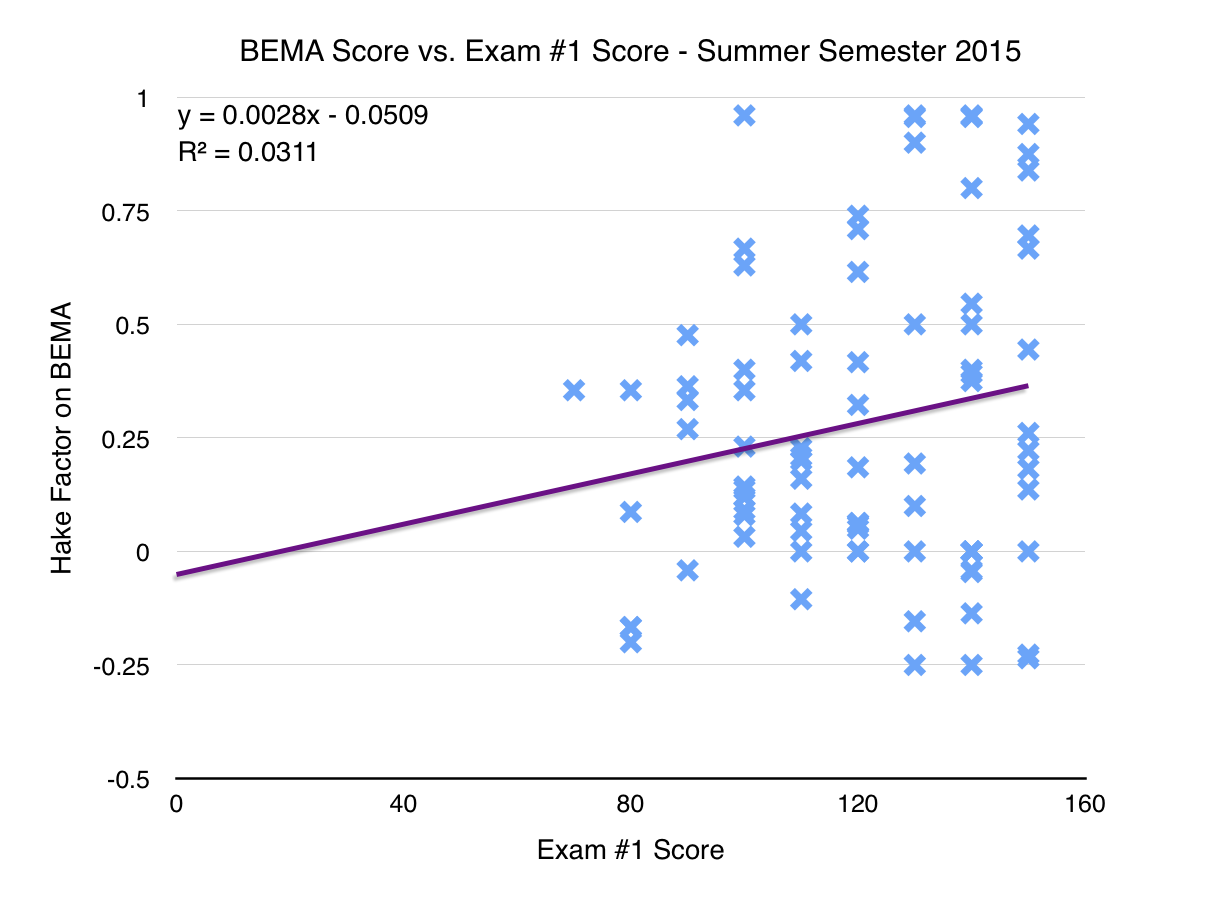
\includegraphics[width=6in]{img/chapter4/bema_vs_ex1_su15}
	\caption[BEMA Hake Factor vs. Exam \#1 Scores]{BEMA Hake Factor vs. Exam \#1 Scores}
  \label{fig:bemaVsExOneSu15}
\end{figure}

\begin{figure}
	\centering
	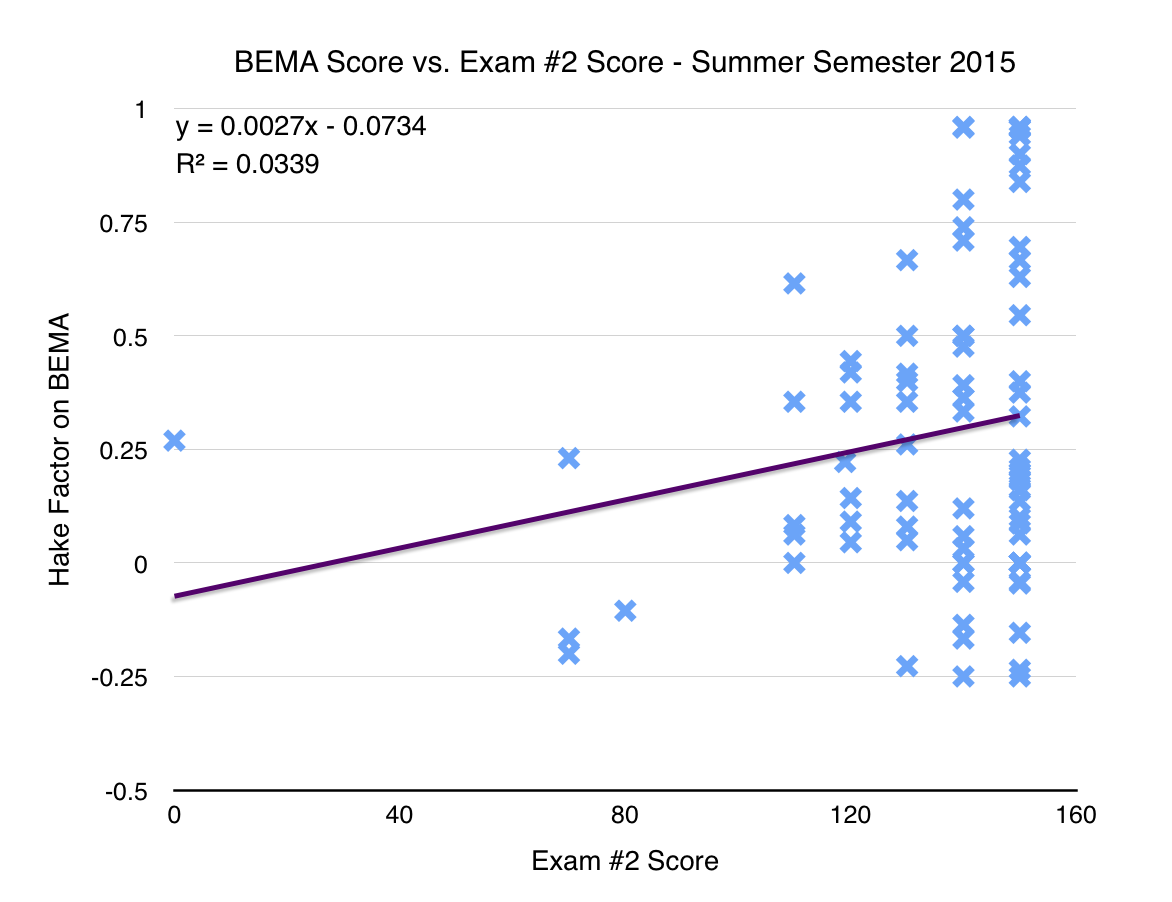
\includegraphics[width=6in]{img/chapter4/bema_vs_ex2_su15}
	\caption[BEMA Hake Factor vs. Exam \#2 Scores]{BEMA Hake Factor vs. Exam \#2 Scores}
  \label{fig:bemaVsExTwoSu15}
\end{figure}

\subsection{Homework Results}

The homework scores yielded very interesting results in this study. One might expect that the inclusion of tutorials would automatically increase the overall score on the homework. However, what I found was quite different. In most cases, the inclusion of the \gls{cita} program did not appreciably affect student problem solving abilities on the homework; scores stayed approximately the same during most semesters. A few times, we see that homework scores were appreciably better during the summer 2015 session (i.e. summer 2015 vs. fall 2014 distance learning) while other times they are worse (i.e. summer 2015 vs. fall 2014).

It is interesting to note that the standard deviation of the summer 2015 class is larger than most of the other classes. This might simply be an artifact of having tested only one class. However, it does merit future investigation.

\begin{figure}
	\centering
	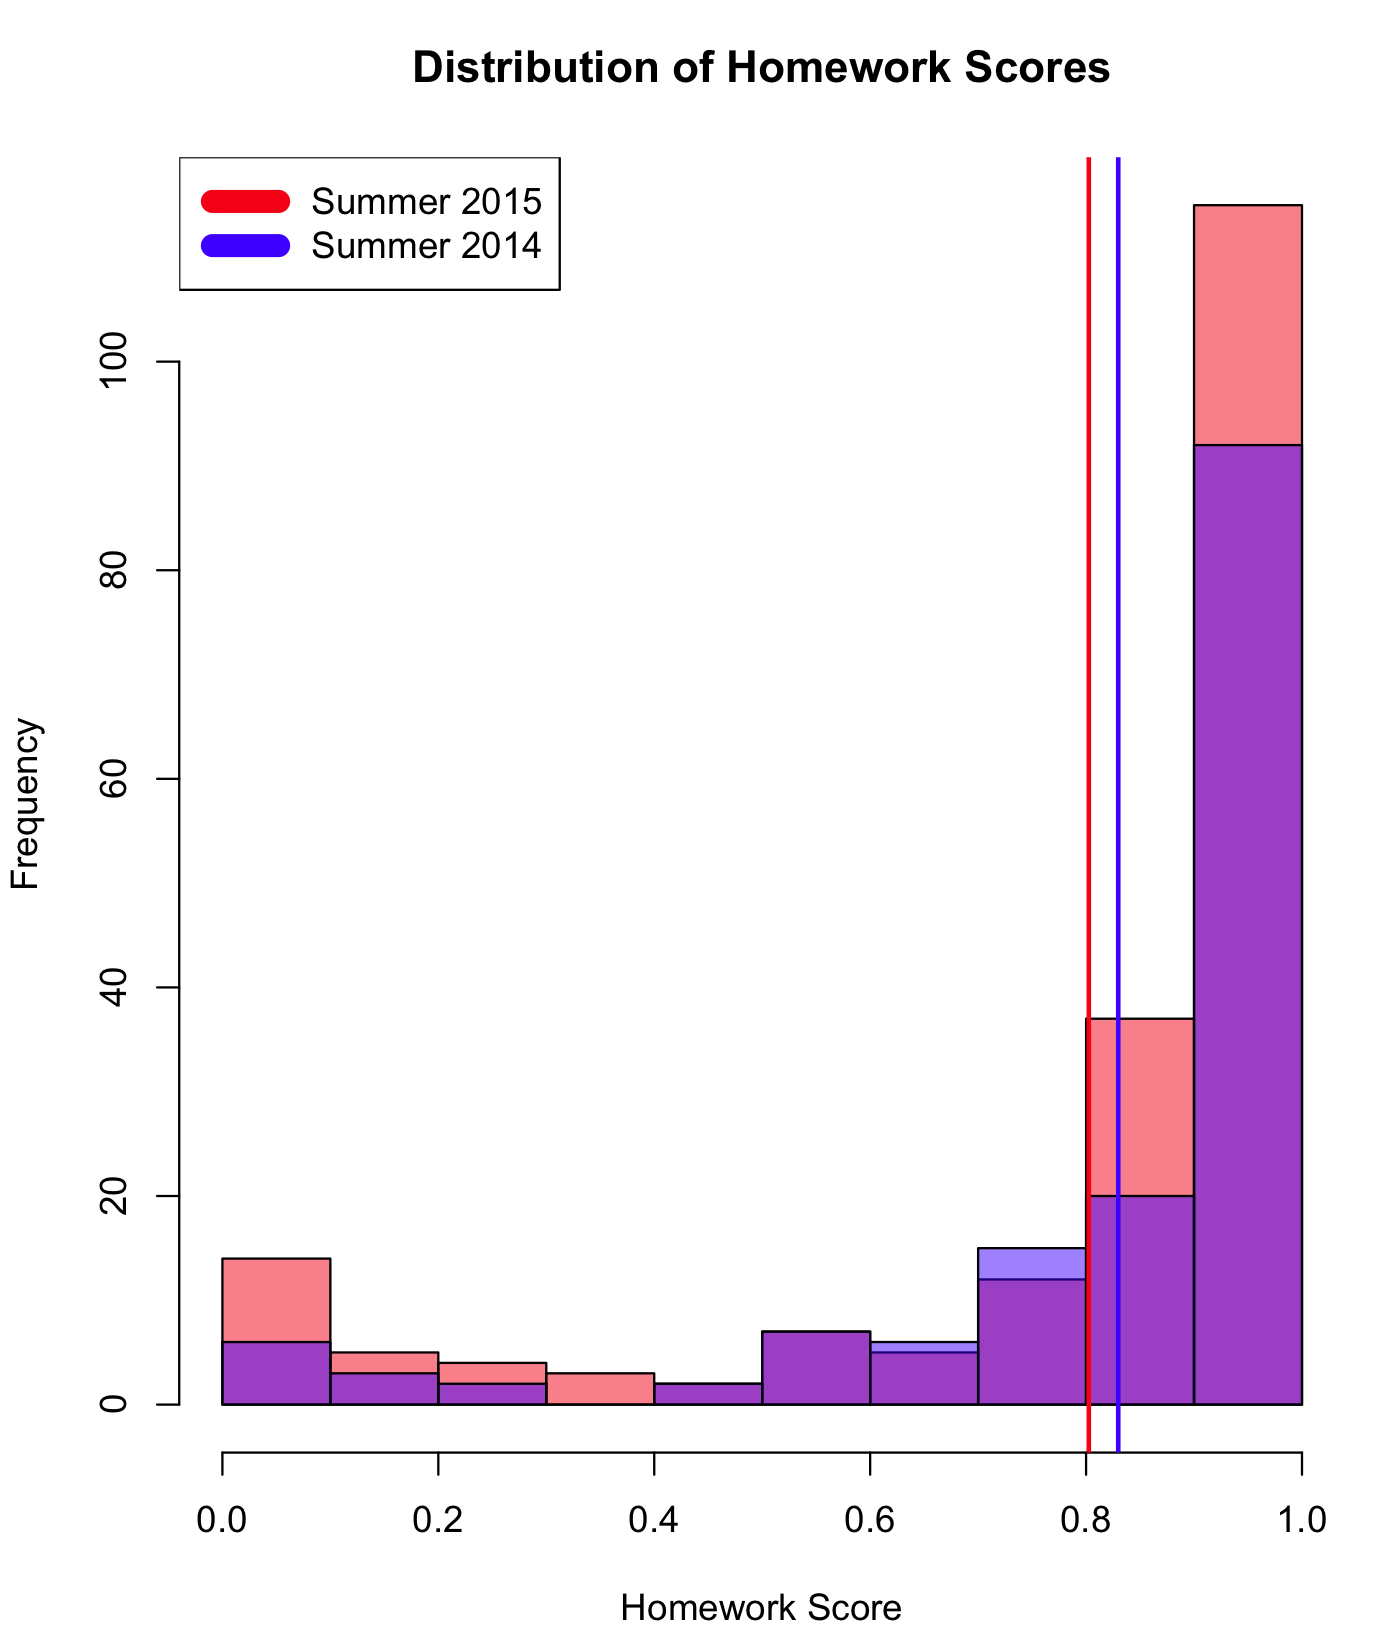
\includegraphics[width=6in]{img/chapter4/hw_su15_vs_su14}
	\caption[Homework Scores (Summer 2014 vs. Summer 2015)]{Homework Scores (Summer 2014 vs. Summer 2015)}
  \label{fig:hwSu14Su15}
\end{figure}

\begin{small}
\begin{table}
  \centering
  \begin{tabular}{|l|l|}
    \hline
    \textbf{Statistic} & \textbf{Value} \\
	\hline
	Mean of Summer 2015 & 0.803 \\
	\hline
	Mean of Summer 2014 & 0.830 \\
	\hline
	Standard Deviation of Summer 2015 & 0.288 \\
	\hline
	Standard Deviation of Summer 2014 & 0.242 \\
	\hline
	Shapiro-Wilk Normality Test of Summer 2015 & p-value $<$ 2.2e-16 \\
	\hline
	Shapiro-Wilk Normality Test of Summer 2014 & p-value $<$ 2.2e-16 \\
	\hline
	Wilcoxon Signed-Rank Test of Homework Scores & p-value = 0.710 \\
	\hline
	Cohen's D of Homework Scores & 0.101 \\
	\hline
  \end{tabular}
	\caption[Homework Scores (Summer 2014 vs. Summer 2015)]{Homework Scores (Summer 2014 vs. Summer 2015)}
  \label{tab:hwSu14Su15}
\end{table}
\end{small}

\begin{figure}
	\centering
	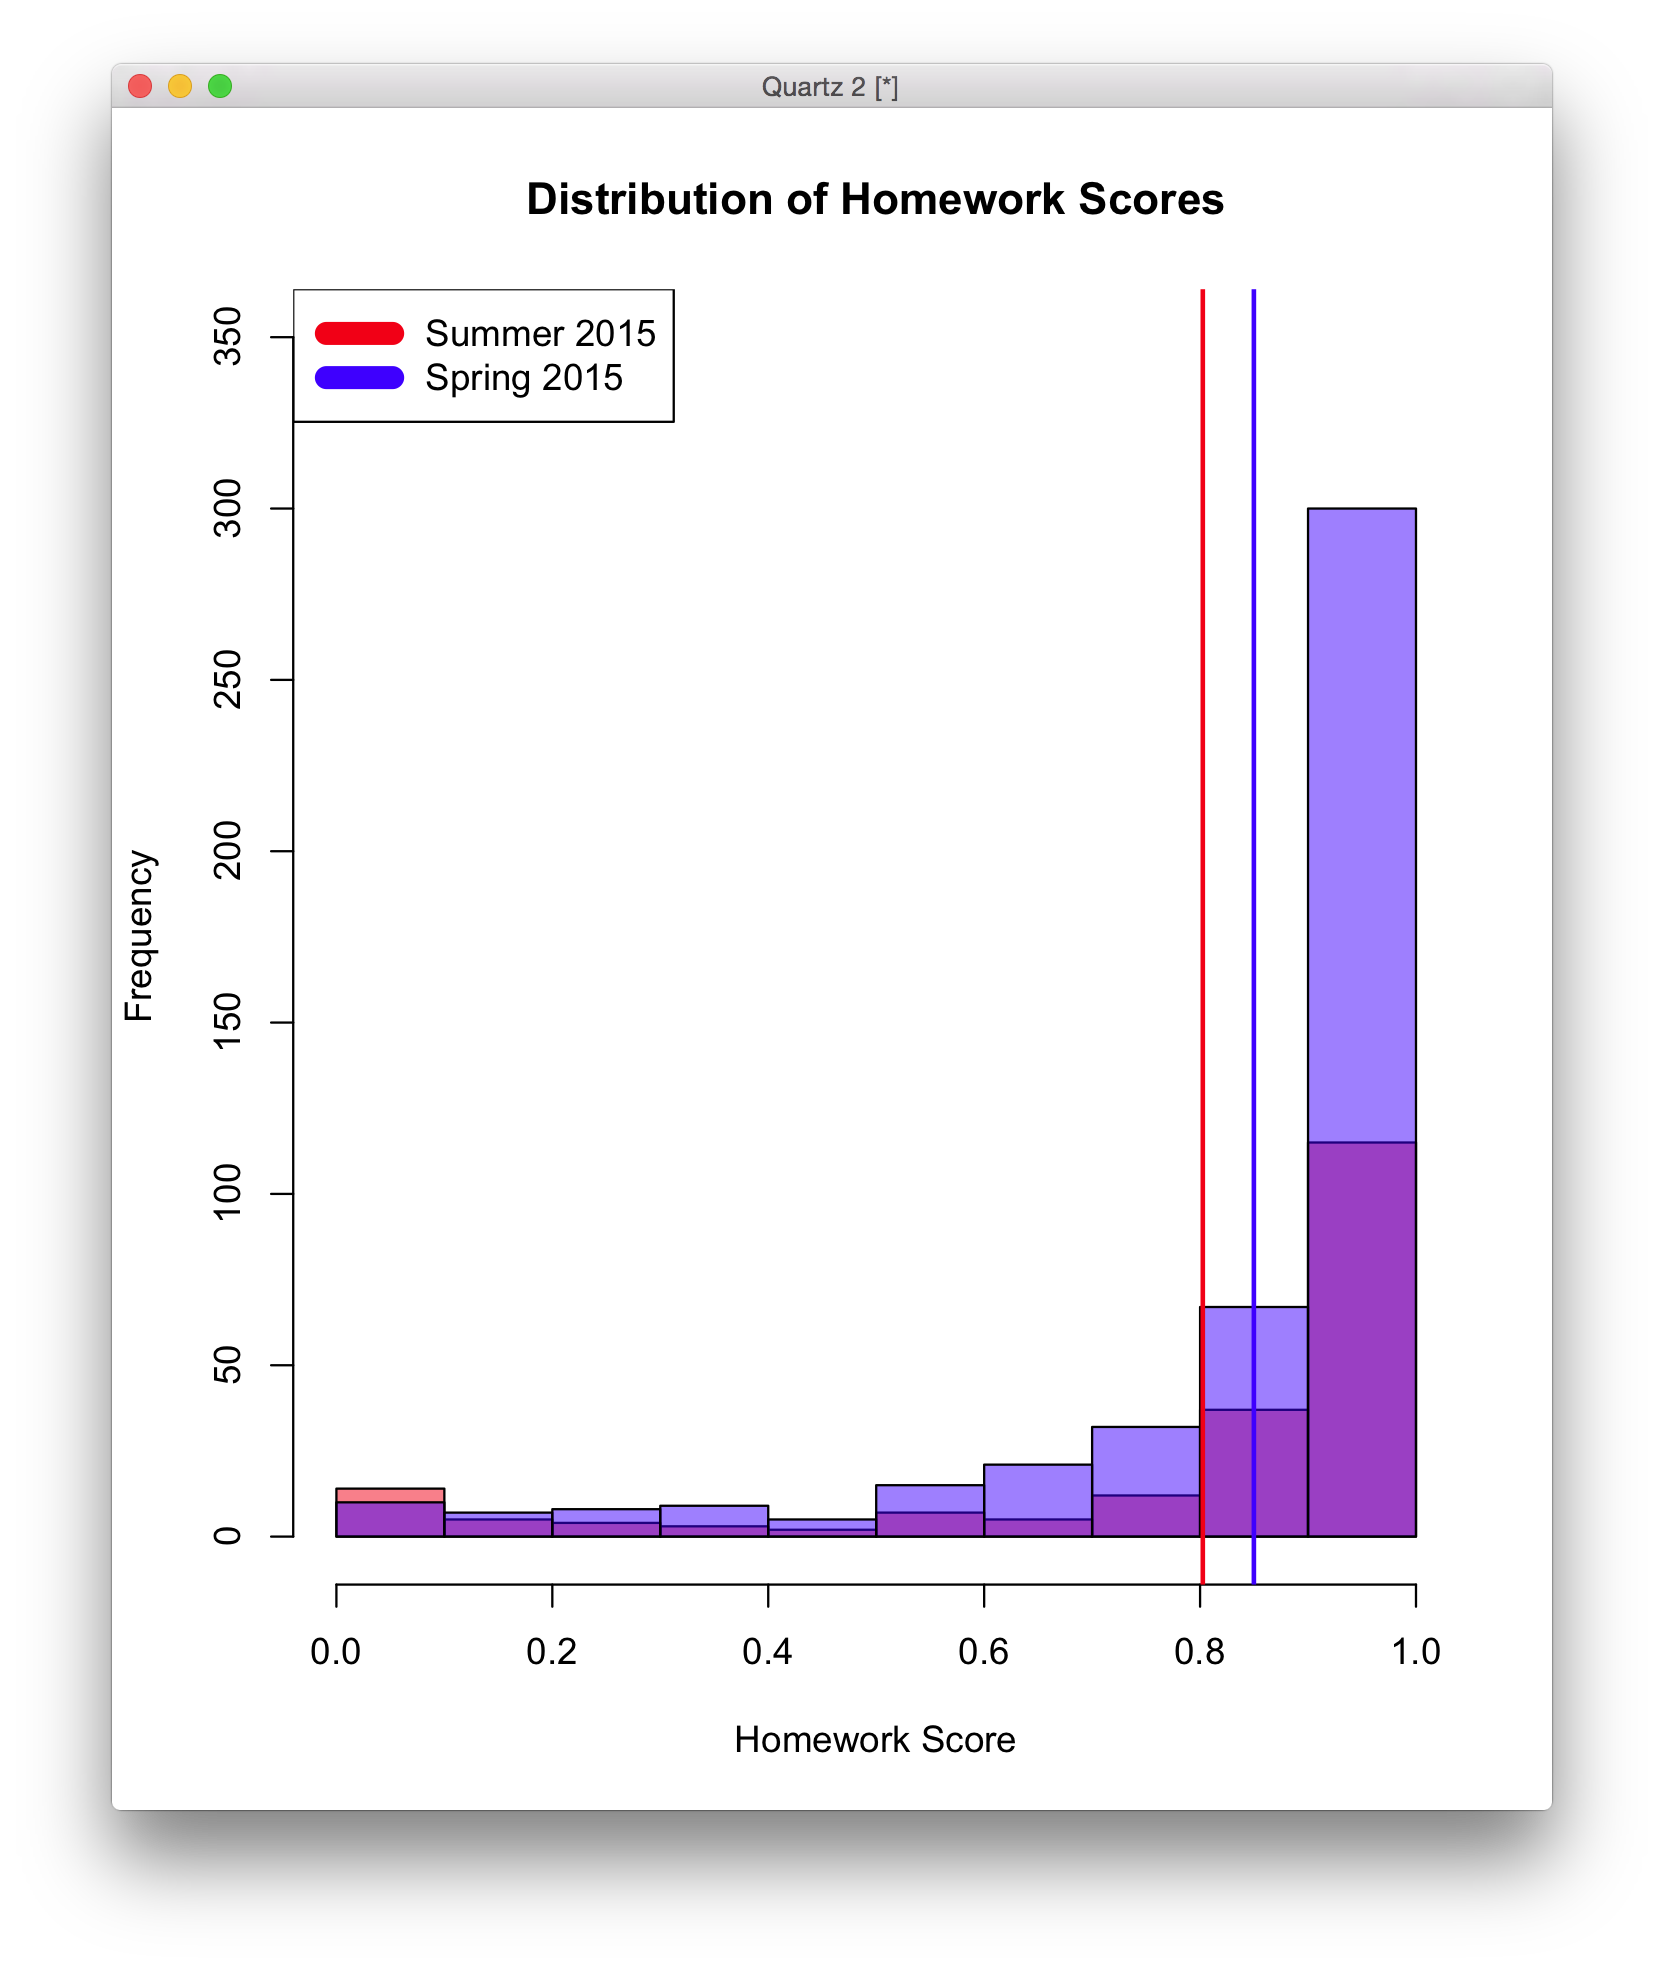
\includegraphics[width=6in]{img/chapter4/hw_su15_vs_sp15}
	\caption[Homework Scores (Spring 2015 vs. Summer 2015)]{Homework Scores (Spring 2015 vs. Summer 2015)}
  \label{fig:hwSu14Su15}
\end{figure}

\begin{small}
\begin{table}
  \centering
  \begin{tabular}{|l|l|}
    \hline
    \textbf{Statistic} & \textbf{Value} \\
	\hline
	Mean of Summer 2015 & 0.803 \\
	\hline
	Mean of Spring 2015 & 0.850 \\
	\hline
	Standard Deviation of Summer 2015 & 0.288 \\
	\hline
	Standard Deviation of Spring 2015 & 0.220 \\
	\hline
	Shapiro-Wilk Normality Test of Summer 2015 & p-value $<$ 2.2e-16 \\
	\hline
	Shapiro-Wilk Normality Test of Spring 2015 & p-value $<$ 2.2e-16 \\
	\hline
	Wilcoxon Signed-Rank Test of Homework Scores & p-value = 0.4551 \\
	\hline
	Cohen's D of Homework Scores & 0.195 \\
	\hline
  \end{tabular}
	\caption[Homework Scores (Spring 2015 vs. Summer 2015)]{Homework Scores (Spring 2015 vs. Summer 2015)}
  \label{fig:hwSu14Su15}
\end{table}
\end{small}

\begin{figure}
	\centering
	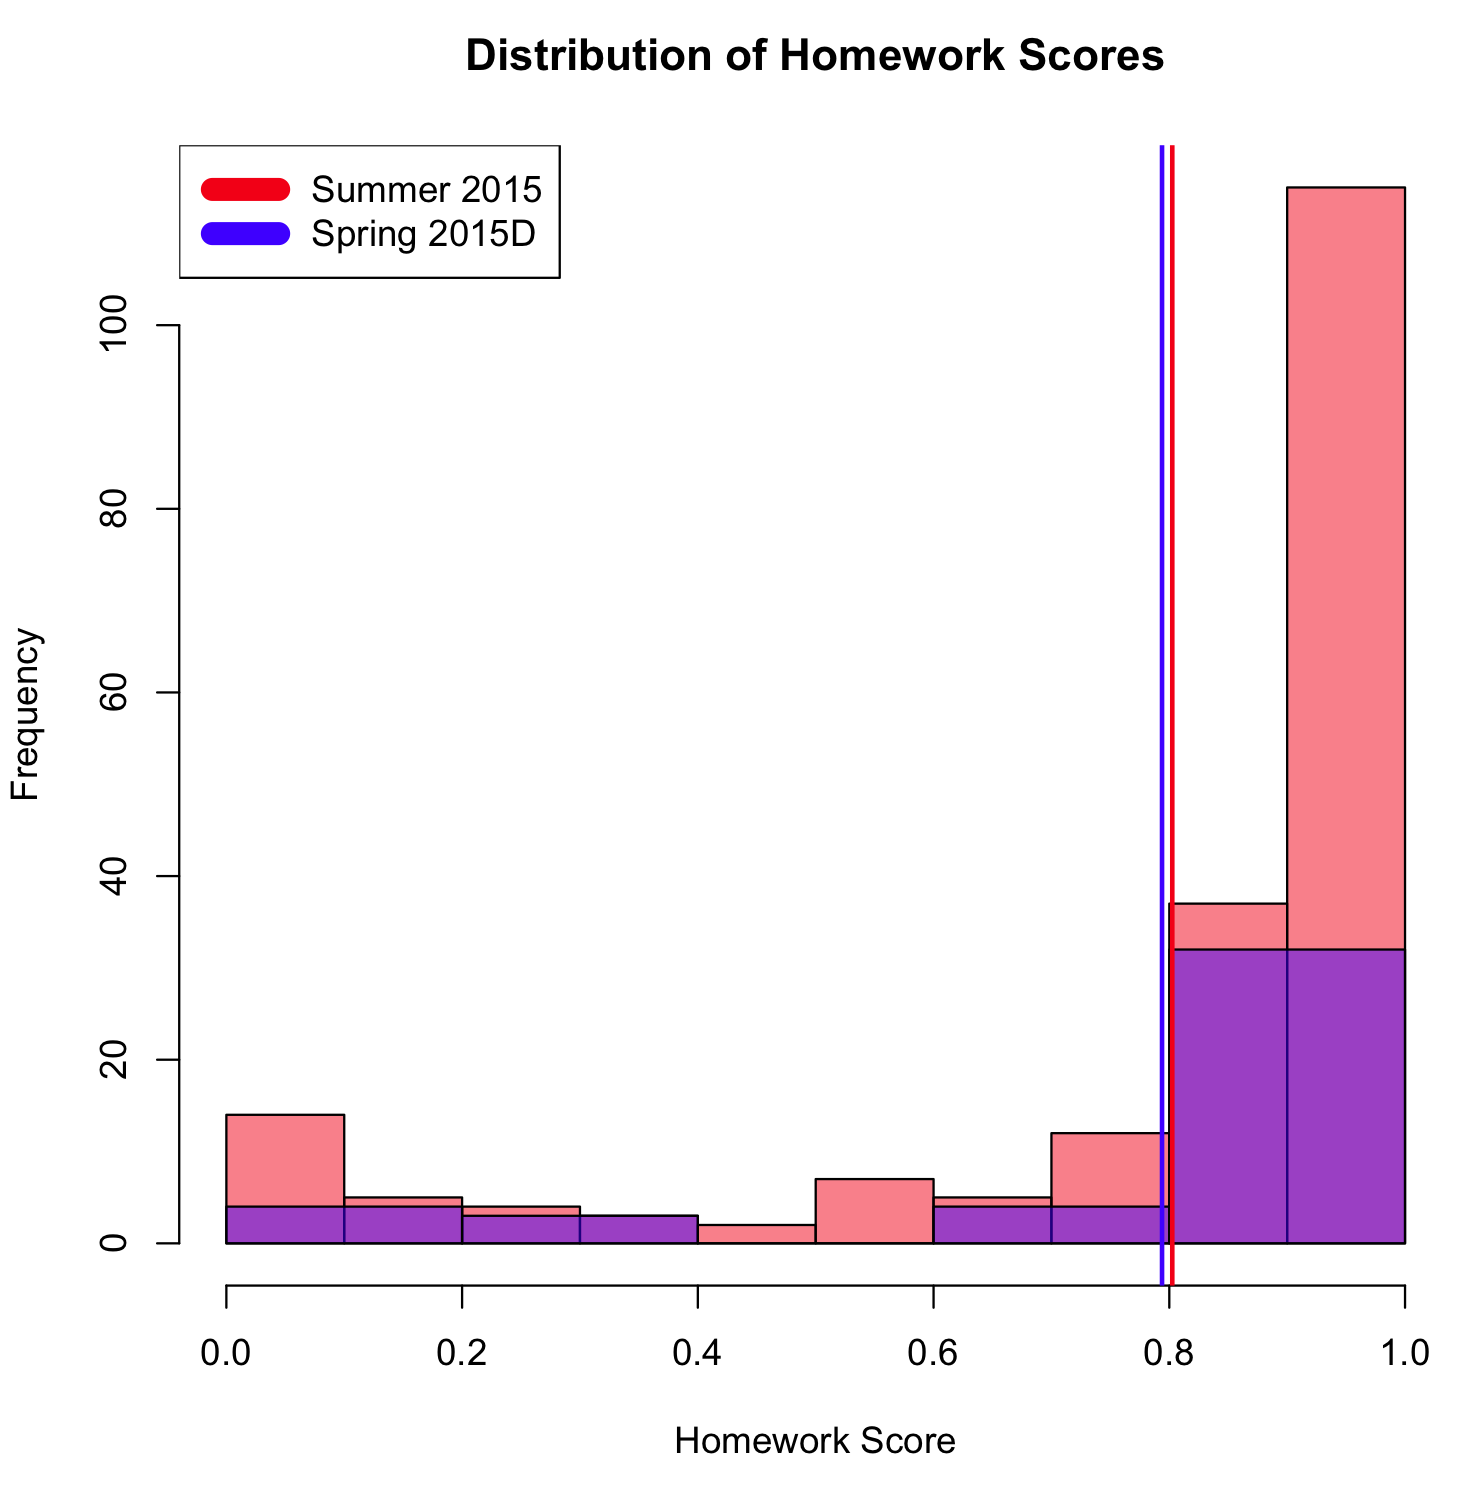
\includegraphics[width=6in]{img/chapter4/hw_su15_vs_sp15d}
	\caption[Homework Scores (Spring 2015 - Distance Learning vs. Summer 2015)]{Homework Scores (Spring 2015 - Distance Learning vs. Summer 2015)}
  \label{fig:hwSu14Su15}
\end{figure}

\begin{small}
\begin{table}
  \centering
  \begin{tabular}{|l|l|}
    \hline
    \textbf{Statistic} & \textbf{Value} \\
	\hline
	Mean of Summer 2015 & 0.803 \\
	\hline
	Mean of Spring 2015 & 0.794 \\
	\hline
	Standard Deviation of Summer 2015 & 0.288 \\
	\hline
	Standard Deviation of Spring 2015 & 0.294 \\
	\hline
	Shapiro-Wilk Normality Test of Summer 2015 & p-value $<$ 2.2e-16 \\
	\hline
	Shapiro-Wilk Normality Test of Spring 2015 & p-value $<$ 2.166e-08 \\
	\hline
	Wilcoxon Signed-Rank Test of Homework Scores & p-value = 0.7237 \\
	\hline
	Cohen's D of Homework Scores & 0.030 \\
	\hline
  \end{tabular}
	\caption[Homework Scores (Spring 2015 - Distance Learning vs. Summer 2015)]{Homework Scores (Spring 2015 - Distance Learning vs. Summer 2015)}
  \label{fig:hwSu14Su15}
\end{table}
\end{small}

\begin{figure}
	\centering
	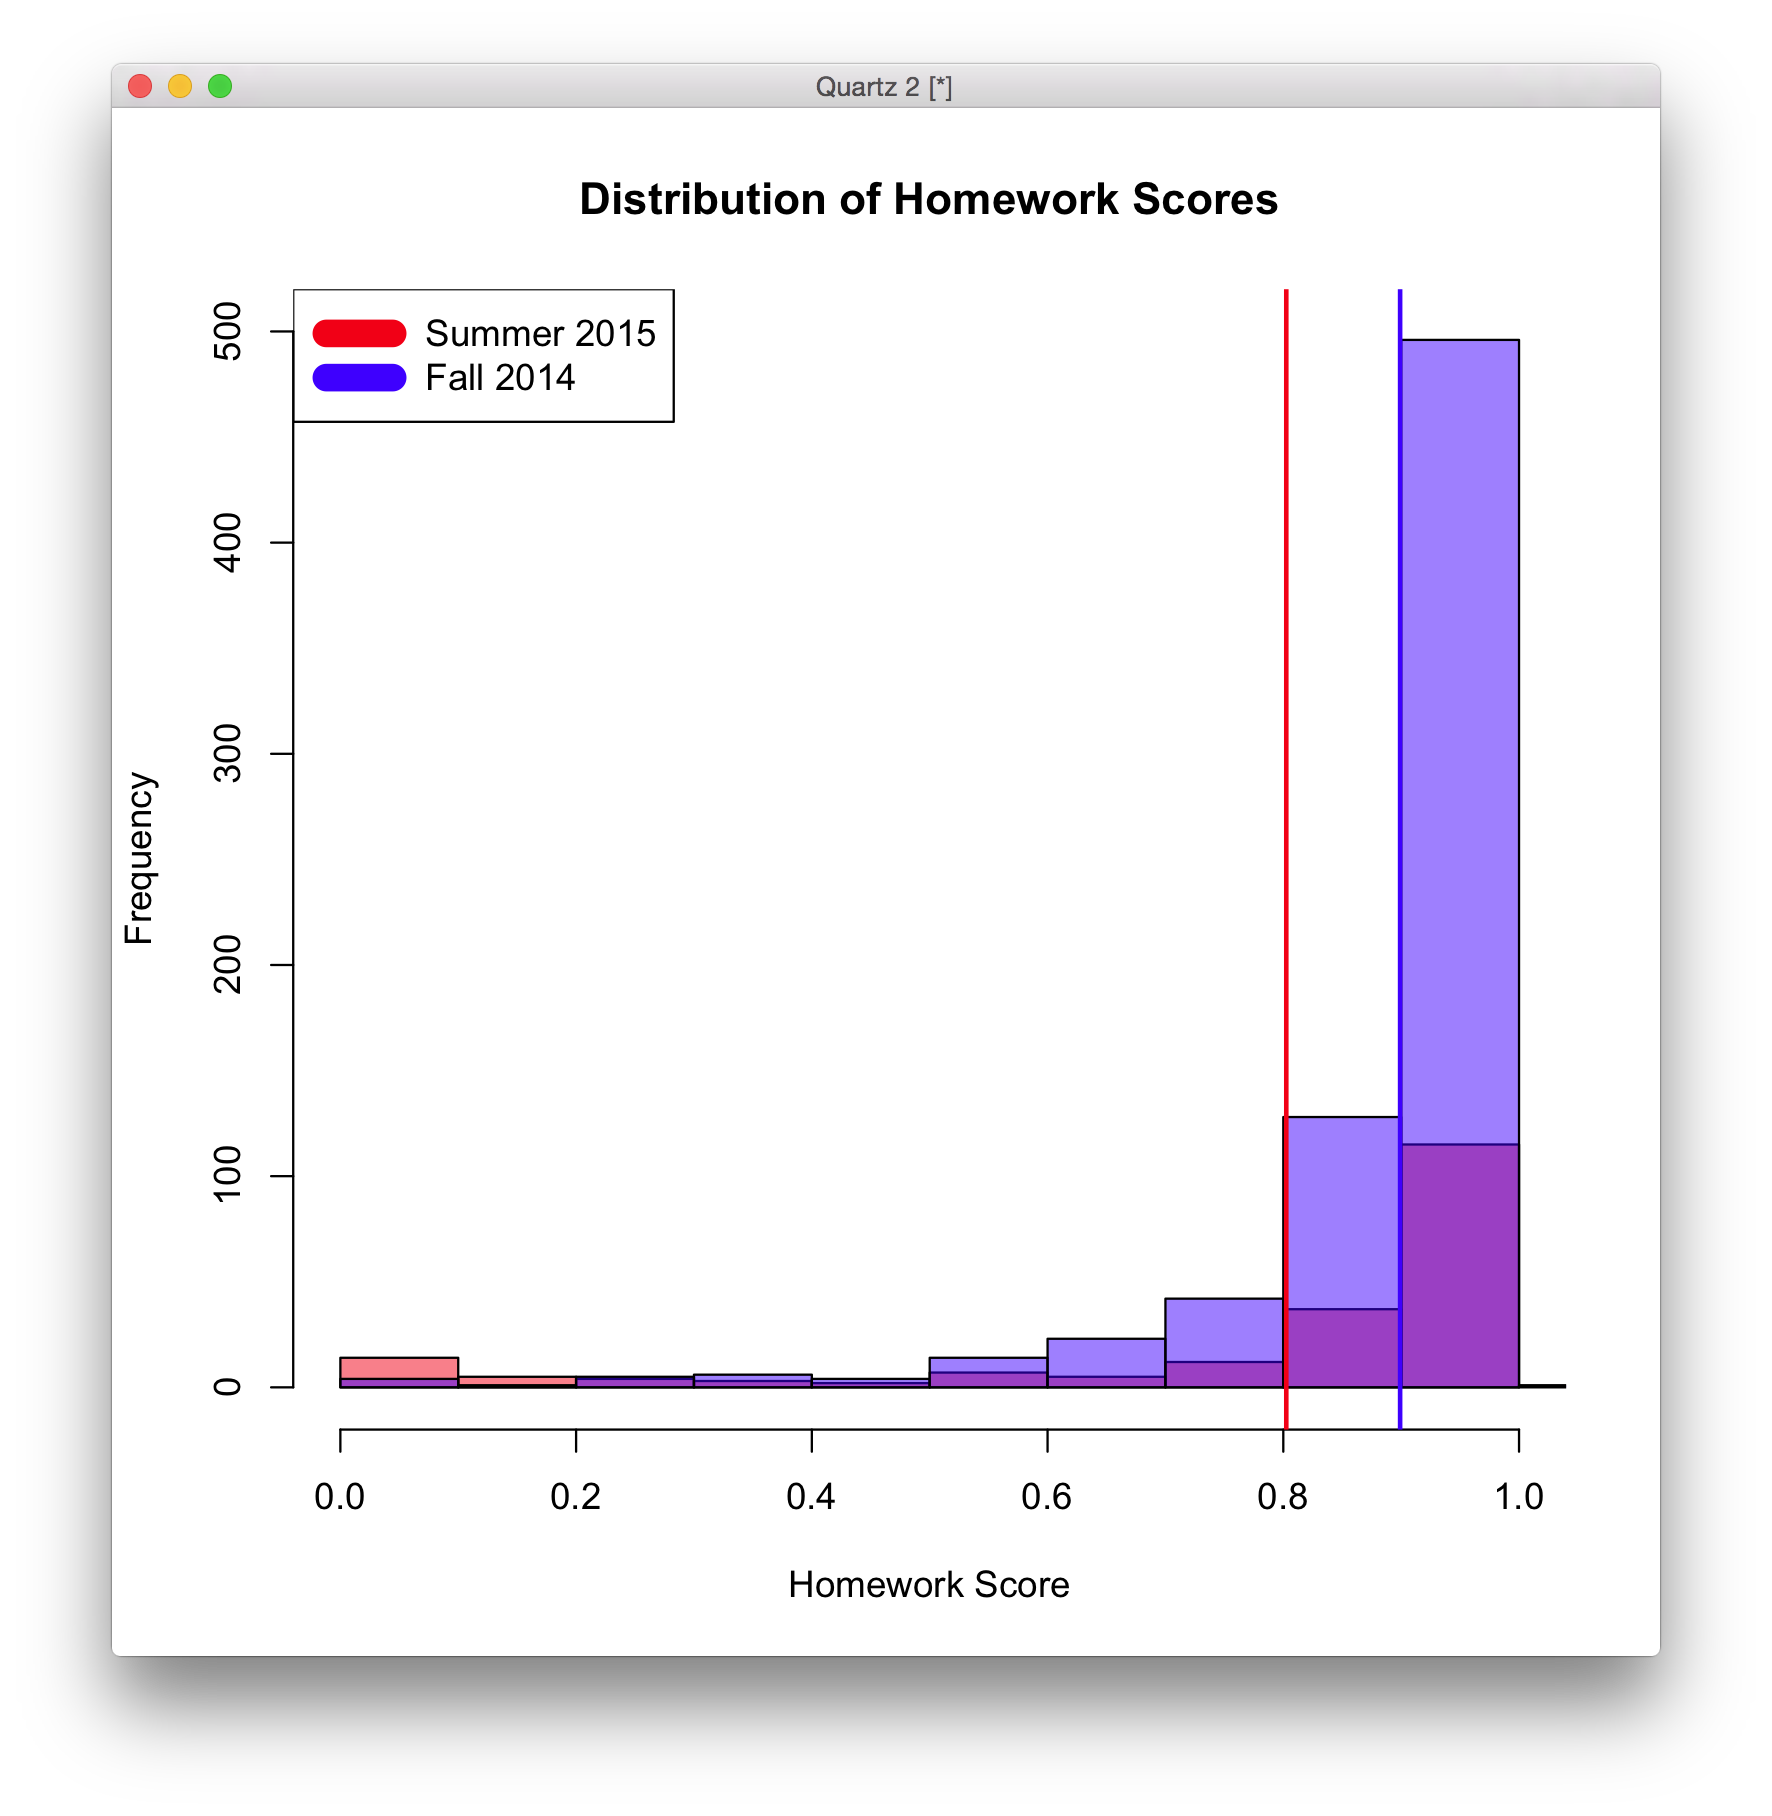
\includegraphics[width=6in]{img/chapter4/hw_su15_vs_f14}
	\caption[Homework Scores (Fall 2014 vs. Summer 2015)]{Homework Scores (Fall 2014 vs. Summer 2015)}
  \label{fig:hwSu14Su15}
\end{figure}

\begin{small}
\begin{table}
  \centering
  \begin{tabular}{|l|l|}
    \hline
    \textbf{Statistic} & \textbf{Value} \\
	\hline
	Mean of Summer 2015 & 0.803 \\
	\hline
	Mean of Fall 2014 & 0.899 \\
	\hline
	Standard Deviation of Summer 2015 & 0.288 \\
	\hline
	Standard Deviation of Spring 2015 & 0.144 \\
	\hline
	Shapiro-Wilk Normality Test of Summer 2015 & p-value $<$ 2.2e-16 \\
	\hline
	Shapiro-Wilk Normality Test of Spring 2015 & p-value $<$ 2.2e-16 \\
	\hline
	Wilcoxon Signed-Rank Test of Homework Scores & p-value = 0.012 \\
	\hline
	Cohen's D of Homework Scores & 0.5212 \\
	\hline
  \end{tabular}
	\caption[Homework Scores (Fall 2014 vs. Summer 2015)]{Homework Scores (Fall 2014 vs. Summer 2015)}
  \label{fig:hwSu14Su15}
\end{table}
\end{small}

\begin{figure}
	\centering
	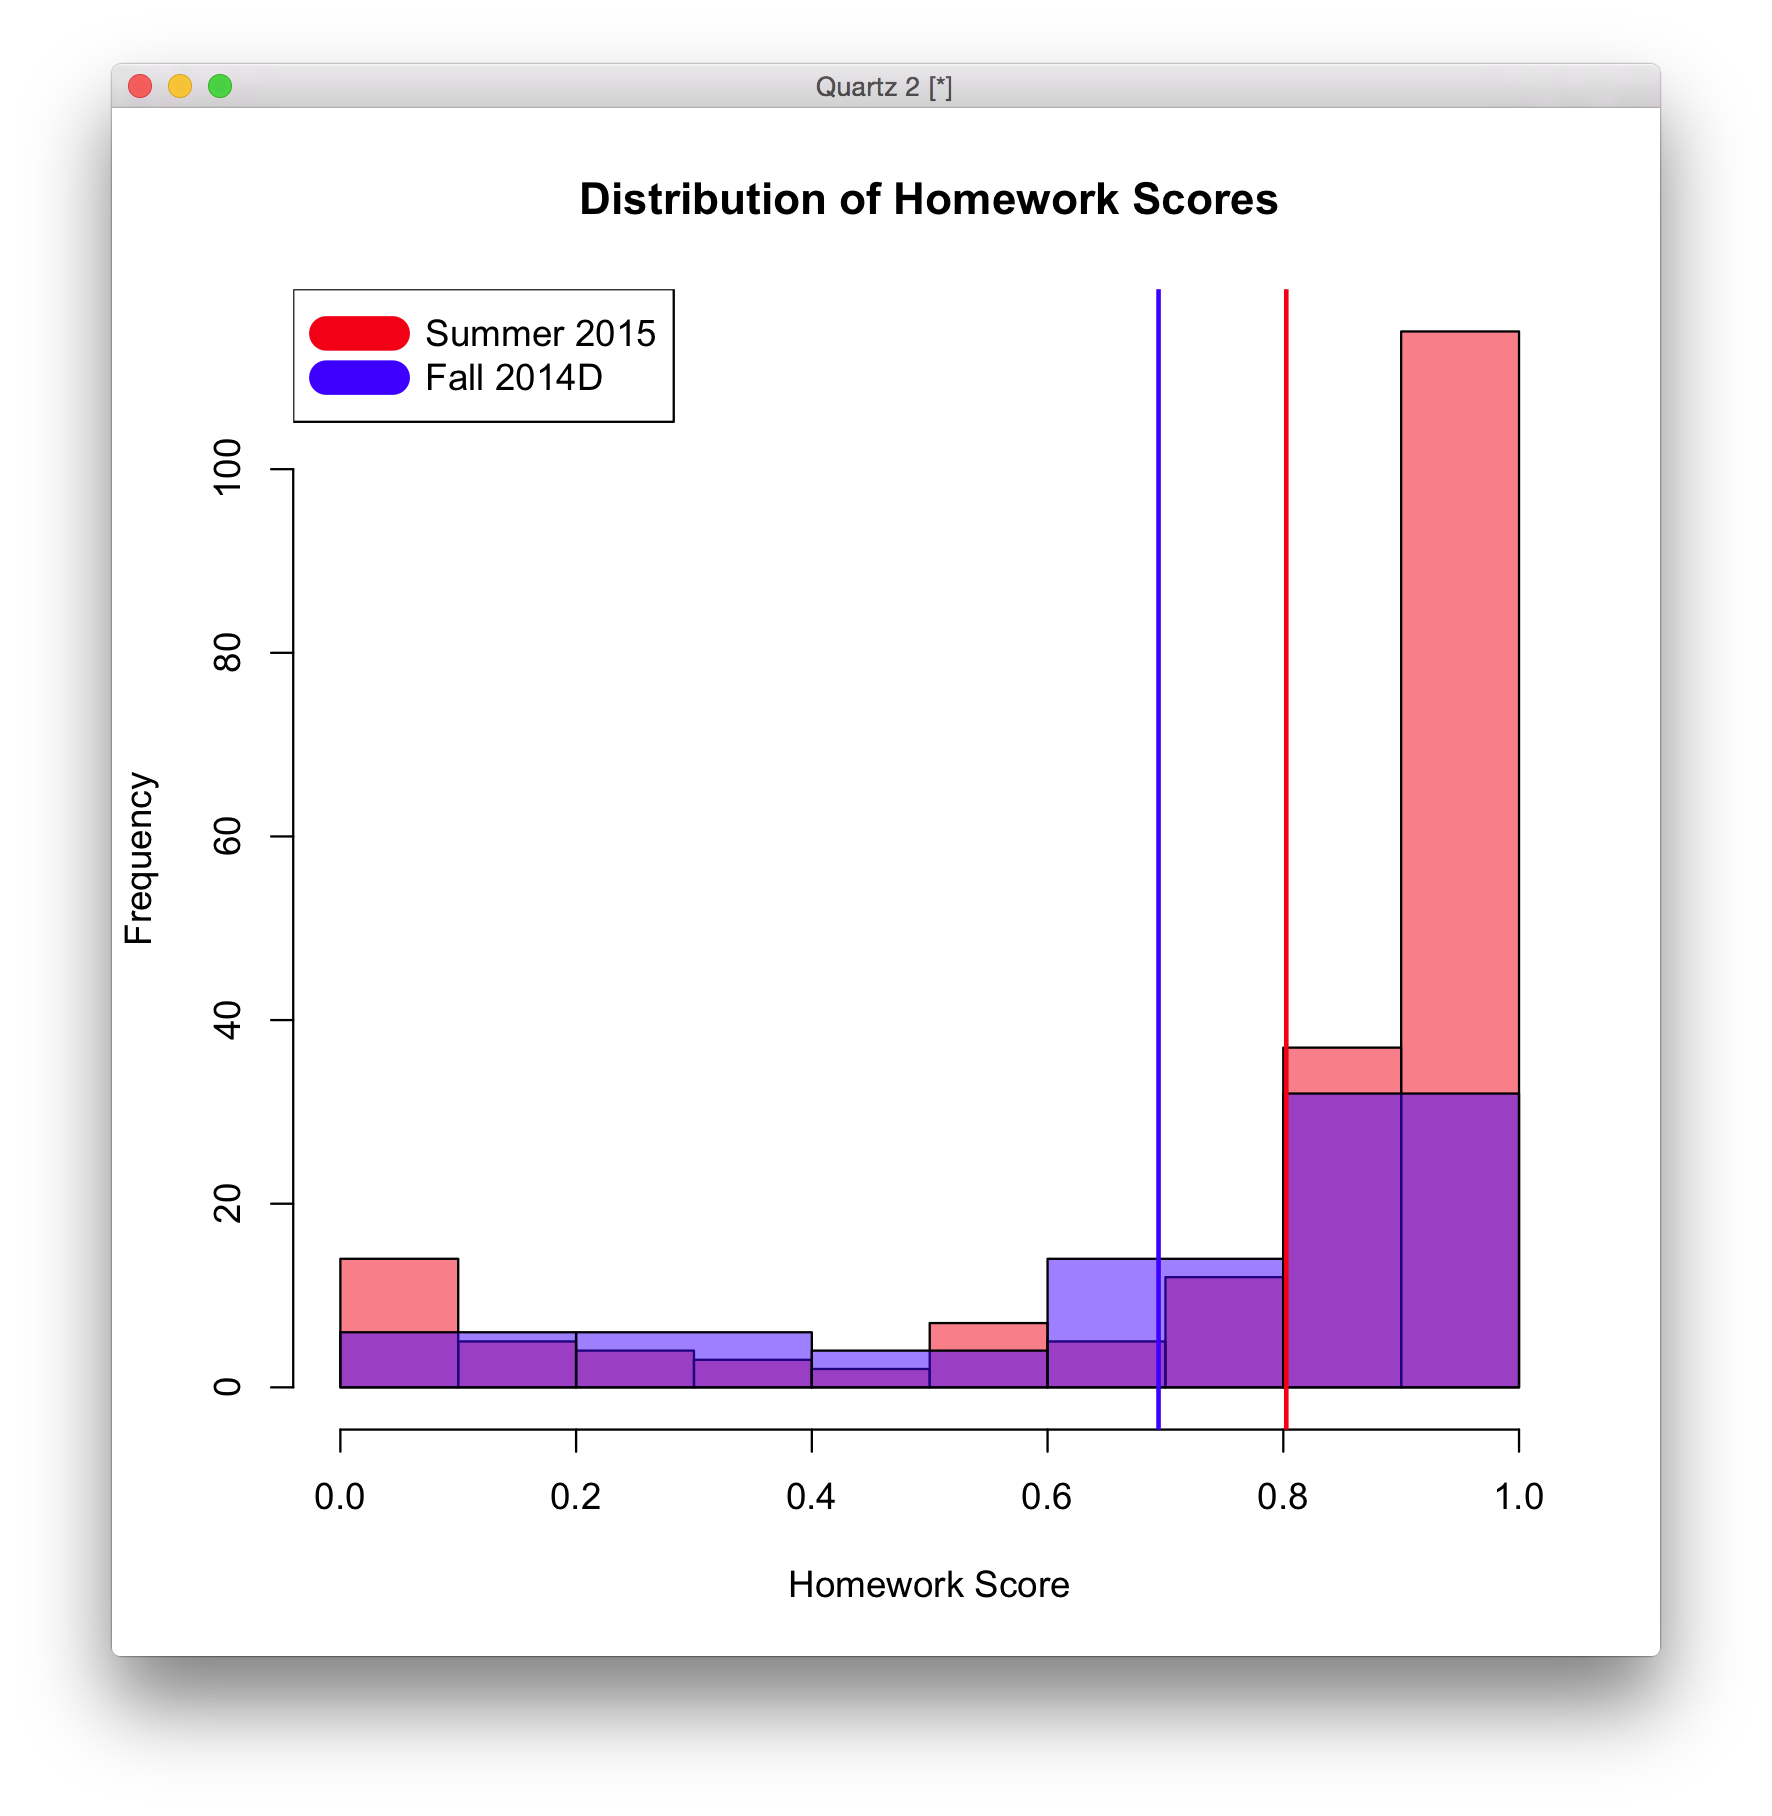
\includegraphics[width=6in]{img/chapter4/hw_su15_vs_f14d}
	\caption[Homework Scores (Fall 2014 - Distance Learning vs. Summer 2015)]{Homework Scores (Fall 2014 - Distance Learning vs. Summer 2015)}
  \label{fig:hwSu14Su15}
\end{figure}

\begin{small}
\begin{table}
  \centering
  \begin{tabular}{|l|l|}
    \hline
    \textbf{Statistic} & \textbf{Value} \\
	\hline
	Mean of Summer 2015 & 0.803 \\
	\hline
	Mean of Fall 2014 & 0.694 \\
	\hline
	Standard Deviation of Summer 2015 & 0.288 \\
	\hline
	Standard Deviation of Spring 2015 & 0.296 \\
	\hline
	Shapiro-Wilk Normality Test of Summer 2015 & p-value $<$ 2.2e-16 \\
	\hline
	Shapiro-Wilk Normality Test of Spring 2015 & p-value $<$ 9.146e-07 \\
	\hline
	Wilcoxon Signed-Rank Test of Homework Scores & p-value = 3.726e-05 \\
	\hline
	Cohen's D of Homework Scores & 0.374 \\
	\hline
  \end{tabular}
	\caption[Homework Scores (Fall 2014 - Distance Learning vs. Summer 2015)]{Homework Scores (Fall 2014 - Distance Learning vs. Summer 2015)}
  \label{fig:hwSu14Su15}
\end{table}
\end{small}

\section{Conclusions}

Due to the gains in score data from above, we predict that student performance is postively affected by the \gls{cita} system. However, it is still too early to make any definitive conclusions. More testing is needed to see how the \gls{cita} system affects student learning.

\section{Future Work}

We plan to conduct our first focus group sessions and student interviews in the fall 2015 semester. Additionally, the research team plans to administer and grade the multi-step problem to on-campus sections of PHYS 24100 starting in the fall 2015 semester. Finally, starting in fall 2015 we would also like to study homework, quiz, and \gls{bema} scores on a question-by-question basis. This will allow us to find trends in the data to figure out which concepts specifically students are having the most trouble on.

The summer 2015 semester of PHYS 24100 will take their final exams during the week August 3, 2015. Thus, the analysis of their exit survey data, end-of-the-semester feedback, final exam data, and final grade data will be deferred to the fall 2015 semester.
